\documentclass[10pt,a4paper,english]{article}\usepackage[]{graphicx}\usepackage[]{color}
%% maxwidth is the original width if it is less than linewidth
%% otherwise use linewidth (to make sure the graphics do not exceed the margin)
\makeatletter
\def\maxwidth{ %
  \ifdim\Gin@nat@width>\linewidth
    \linewidth
  \else
    \Gin@nat@width
  \fi
}
\makeatother

\definecolor{fgcolor}{rgb}{0.345, 0.345, 0.345}
\newcommand{\hlnum}[1]{\textcolor[rgb]{0.686,0.059,0.569}{#1}}%
\newcommand{\hlstr}[1]{\textcolor[rgb]{0.192,0.494,0.8}{#1}}%
\newcommand{\hlcom}[1]{\textcolor[rgb]{0.678,0.584,0.686}{\textit{#1}}}%
\newcommand{\hlopt}[1]{\textcolor[rgb]{0,0,0}{#1}}%
\newcommand{\hlstd}[1]{\textcolor[rgb]{0.345,0.345,0.345}{#1}}%
\newcommand{\hlkwa}[1]{\textcolor[rgb]{0.161,0.373,0.58}{\textbf{#1}}}%
\newcommand{\hlkwb}[1]{\textcolor[rgb]{0.69,0.353,0.396}{#1}}%
\newcommand{\hlkwc}[1]{\textcolor[rgb]{0.333,0.667,0.333}{#1}}%
\newcommand{\hlkwd}[1]{\textcolor[rgb]{0.737,0.353,0.396}{\textbf{#1}}}%
\let\hlipl\hlkwb

\usepackage{framed}
\makeatletter
\newenvironment{kframe}{%
 \def\at@end@of@kframe{}%
 \ifinner\ifhmode%
  \def\at@end@of@kframe{\end{minipage}}%
  \begin{minipage}{\columnwidth}%
 \fi\fi%
 \def\FrameCommand##1{\hskip\@totalleftmargin \hskip-\fboxsep
 \colorbox{shadecolor}{##1}\hskip-\fboxsep
     % There is no \\@totalrightmargin, so:
     \hskip-\linewidth \hskip-\@totalleftmargin \hskip\columnwidth}%
 \MakeFramed {\advance\hsize-\width
   \@totalleftmargin\z@ \linewidth\hsize
   \@setminipage}}%
 {\par\unskip\endMakeFramed%
 \at@end@of@kframe}
\makeatother

\definecolor{shadecolor}{rgb}{.97, .97, .97}
\definecolor{messagecolor}{rgb}{0, 0, 0}
\definecolor{warningcolor}{rgb}{1, 0, 1}
\definecolor{errorcolor}{rgb}{1, 0, 0}
\newenvironment{knitrout}{}{} % an empty environment to be redefined in TeX

\usepackage{alltt}

% now ignored, I think:
%\VignetteEngine{knitr::knitr}
%\VignetteIndexEntry{Asymptotic Distribution of the Markowitz Portfolio}
%\VignetteKeyword{Finance}
%\VignetteKeyword{Markowitz}
%\VignettePackage{MarkowitzR}

\batchmode

% front matter%FOLDUP
\usepackage[hyphens]{url}
\usepackage{amsmath}
\usepackage{amsfonts}
% for therefore
\usepackage{amssymb}
% for theorems?
\usepackage{amsthm}

\theoremstyle{plain}
\newtheorem{theorem}{Theorem}[section]
\newtheorem{lemma}[theorem]{Lemma}
\newtheorem{corollary}[theorem]{Corollary}

\theoremstyle{definition}
\newtheorem{definition}[theorem]{Definition}
\newtheorem{conjecture}[theorem]{Conjecture}
\newtheorem{assumption}[theorem]{Assumption}
\newtheorem{example}{Example}[section]

\theoremstyle{remark}
\newtheorem*{remark}{Remark}
\newtheorem*{caution}{Caution}
\newtheorem*{note}{Note}

% see http://tex.stackexchange.com/a/3034/2530
\PassOptionsToPackage{hyphens}{url}\usepackage{hyperref}
\usepackage{hyperref}
\usepackage[square,numbers]{natbib}
%\usepackage[authoryear]{natbib}
%\usepackage[iso]{datetime}
%\usepackage{datetime}
\usepackage{gitinfo2}

%%http://choorucode.com/2010/05/05/how-to-add-draft-watermark-in-latex/
%\usepackage{draftwatermark}
%% V1 sent to Mortada.
%% V2 on paper to JHZD.
%% V3 sent to s.lee@BR 140826
%\providecommand{\versnum}{V4}
%\SetWatermarkText{DRAFT \versnum}
%\SetWatermarkLightness{0.87}
%\SetWatermarkScale{4.5}

%\usepackage{fancyhdr}
%\pagestyle{fancy}
%\chead{}
%\rhead{}
%\lhead{}
%\rhead{\sc draft \versnum; do not distribute}
%\rfoot{}

%compactitem and such:
\usepackage[newitem,newenum,increaseonly]{paralist}

\makeatletter
\makeatother

% see https://www.overleaf.com/blog/619-tip-of-the-week-add-inline-or-margin-comments-to-your-pdf#.Wk26SN-YWXI
\usepackage[colorinlistoftodos]{todonotes}
% for release, disable them!
%\usepackage[disable]{todonotes}

%\input{sr_defs.tex}
\usepackage[notheorems]{SharpeR}

\providecommand{\sideWarning}[1][0.5]{\marginpar{\hfill\includegraphics[width=#1\marginparwidth]{warning}}}

% knitr setup%FOLDUP


%UNFOLD


    
% SYMPY preamble%FOLDUP
    
    %\usepackage{graphicx} % Used to insert images
    %\usepackage{adjustbox} % Used to constrain images to a maximum size 
    \usepackage{color} % Allow colors to be defined
    \usepackage{enumerate} % Needed for markdown enumerations to work
    %\usepackage{geometry} % Used to adjust the document margins
    \usepackage{amsmath} % Equations
    \usepackage{amssymb} % Equations
    %\usepackage[utf8]{inputenc} % Allow utf-8 characters in the tex document
    %\usepackage[mathletters]{ucs} % Extended unicode (utf-8) support
		\usepackage{fancyvrb} % verbatim replacement that allows latex
    %\usepackage{grffile} % extends the file name processing of package graphics 
                         % to support a larger range 
    % The hyperref package gives us a pdf with properly built
    % internal navigation ('pdf bookmarks' for the table of contents,
    % internal cross-reference links, web links for URLs, etc.)
    \usepackage{hyperref}
    %\usepackage{longtable} % longtable support required by pandoc >1.10
    

    
    
    \definecolor{orange}{cmyk}{0,0.4,0.8,0.2}
    \definecolor{darkorange}{rgb}{.71,0.21,0.01}
    \definecolor{darkgreen}{rgb}{.12,.54,.11}
    \definecolor{myteal}{rgb}{.26, .44, .56}
    \definecolor{gray}{gray}{0.45}
    \definecolor{lightgray}{gray}{.95}
    \definecolor{mediumgray}{gray}{.8}
    \definecolor{inputbackground}{rgb}{.95, .95, .85}
    \definecolor{outputbackground}{rgb}{.95, .95, .95}
    \definecolor{traceback}{rgb}{1, .95, .95}
    % ansi colors
    \definecolor{red}{rgb}{.6,0,0}
    \definecolor{green}{rgb}{0,.65,0}
    \definecolor{brown}{rgb}{0.6,0.6,0}
    \definecolor{blue}{rgb}{0,.145,.698}
    \definecolor{purple}{rgb}{.698,.145,.698}
    \definecolor{cyan}{rgb}{0,.698,.698}
    \definecolor{lightgray}{gray}{0.5}
    
    % bright ansi colors
    \definecolor{darkgray}{gray}{0.25}
    \definecolor{lightred}{rgb}{1.0,0.39,0.28}
    \definecolor{lightgreen}{rgb}{0.48,0.99,0.0}
    \definecolor{lightblue}{rgb}{0.53,0.81,0.92}
    \definecolor{lightpurple}{rgb}{0.87,0.63,0.87}
    \definecolor{lightcyan}{rgb}{0.5,1.0,0.83}
    
    % commands and environments needed by pandoc snippets
    % extracted from the output of `pandoc -s`
    
    %\DefineShortVerb[commandchars=\\\{\}]{\|}
    %\DefineVerbatimEnvironment{Highlighting}{Verbatim}{commandchars=\\\{\}}
    %% Add ',fontsize=\small' for more characters per line
    %\newenvironment{Shaded}{}{}
    %\newcommand{\KeywordTok}[1]{\textcolor[rgb]{0.00,0.44,0.13}{\textbf{{#1}}}}
    %\newcommand{\DataTypeTok}[1]{\textcolor[rgb]{0.56,0.13,0.00}{{#1}}}
    %\newcommand{\DecValTok}[1]{\textcolor[rgb]{0.25,0.63,0.44}{{#1}}}
    %\newcommand{\BaseNTok}[1]{\textcolor[rgb]{0.25,0.63,0.44}{{#1}}}
    %\newcommand{\FloatTok}[1]{\textcolor[rgb]{0.25,0.63,0.44}{{#1}}}
    %\newcommand{\CharTok}[1]{\textcolor[rgb]{0.25,0.44,0.63}{{#1}}}
    %\newcommand{\StringTok}[1]{\textcolor[rgb]{0.25,0.44,0.63}{{#1}}}
    %\newcommand{\CommentTok}[1]{\textcolor[rgb]{0.38,0.63,0.69}{\textit{{#1}}}}
    %\newcommand{\OtherTok}[1]{\textcolor[rgb]{0.00,0.44,0.13}{{#1}}}
    %\newcommand{\AlertTok}[1]{\textcolor[rgb]{1.00,0.00,0.00}{\textbf{{#1}}}}
    %\newcommand{\FunctionTok}[1]{\textcolor[rgb]{0.02,0.16,0.49}{{#1}}}
    %\newcommand{\RegionMarkerTok}[1]{{#1}}
    %\newcommand{\ErrorTok}[1]{\textcolor[rgb]{1.00,0.00,0.00}{\textbf{{#1}}}}
    %\newcommand{\NormalTok}[1]{{#1}}
    
    %% Define a nice break command that doesn't care if a line doesn't already
    %% exist.
    %\def\br{\hspace*{\fill} \\* }
    %% Math Jax compatability definitions
    %\def\gt{>}
    %\def\lt{<}
    

    %% Pygments definitions
    
%\makeatletter
%\def\PY@reset{\let\PY@it=\relax \let\PY@bf=\relax%
    %\let\PY@ul=\relax \let\PY@tc=\relax%
    %\let\PY@bc=\relax \let\PY@ff=\relax}
%\def\PY@tok#1{\csname PY@tok@#1\endcsname}
%\def\PY@toks#1+{\ifx\relax#1\empty\else%
    %\PY@tok{#1}\expandafter\PY@toks\fi}
%\def\PY@do#1{\PY@bc{\PY@tc{\PY@ul{%
    %\PY@it{\PY@bf{\PY@ff{#1}}}}}}}
%\def\PY#1#2{\PY@reset\PY@toks#1+\relax+\PY@do{#2}}

%\expandafter\def\csname PY@tok@gd\endcsname{\def\PY@tc##1{\textcolor[rgb]{0.63,0.00,0.00}{##1}}}
%\expandafter\def\csname PY@tok@gu\endcsname{\let\PY@bf=\textbf\def\PY@tc##1{\textcolor[rgb]{0.50,0.00,0.50}{##1}}}
%\expandafter\def\csname PY@tok@gt\endcsname{\def\PY@tc##1{\textcolor[rgb]{0.00,0.27,0.87}{##1}}}
%\expandafter\def\csname PY@tok@gs\endcsname{\let\PY@bf=\textbf}
%\expandafter\def\csname PY@tok@gr\endcsname{\def\PY@tc##1{\textcolor[rgb]{1.00,0.00,0.00}{##1}}}
%\expandafter\def\csname PY@tok@cm\endcsname{\let\PY@it=\textit\def\PY@tc##1{\textcolor[rgb]{0.25,0.50,0.50}{##1}}}
%\expandafter\def\csname PY@tok@vg\endcsname{\def\PY@tc##1{\textcolor[rgb]{0.10,0.09,0.49}{##1}}}
%\expandafter\def\csname PY@tok@m\endcsname{\def\PY@tc##1{\textcolor[rgb]{0.40,0.40,0.40}{##1}}}
%\expandafter\def\csname PY@tok@mh\endcsname{\def\PY@tc##1{\textcolor[rgb]{0.40,0.40,0.40}{##1}}}
%\expandafter\def\csname PY@tok@go\endcsname{\def\PY@tc##1{\textcolor[rgb]{0.53,0.53,0.53}{##1}}}
%\expandafter\def\csname PY@tok@ge\endcsname{\let\PY@it=\textit}
%\expandafter\def\csname PY@tok@vc\endcsname{\def\PY@tc##1{\textcolor[rgb]{0.10,0.09,0.49}{##1}}}
%\expandafter\def\csname PY@tok@il\endcsname{\def\PY@tc##1{\textcolor[rgb]{0.40,0.40,0.40}{##1}}}
%\expandafter\def\csname PY@tok@cs\endcsname{\let\PY@it=\textit\def\PY@tc##1{\textcolor[rgb]{0.25,0.50,0.50}{##1}}}
%\expandafter\def\csname PY@tok@cp\endcsname{\def\PY@tc##1{\textcolor[rgb]{0.74,0.48,0.00}{##1}}}
%\expandafter\def\csname PY@tok@gi\endcsname{\def\PY@tc##1{\textcolor[rgb]{0.00,0.63,0.00}{##1}}}
%\expandafter\def\csname PY@tok@gh\endcsname{\let\PY@bf=\textbf\def\PY@tc##1{\textcolor[rgb]{0.00,0.00,0.50}{##1}}}
%\expandafter\def\csname PY@tok@ni\endcsname{\let\PY@bf=\textbf\def\PY@tc##1{\textcolor[rgb]{0.60,0.60,0.60}{##1}}}
%\expandafter\def\csname PY@tok@nl\endcsname{\def\PY@tc##1{\textcolor[rgb]{0.63,0.63,0.00}{##1}}}
%\expandafter\def\csname PY@tok@nn\endcsname{\let\PY@bf=\textbf\def\PY@tc##1{\textcolor[rgb]{0.00,0.00,1.00}{##1}}}
%\expandafter\def\csname PY@tok@no\endcsname{\def\PY@tc##1{\textcolor[rgb]{0.53,0.00,0.00}{##1}}}
%\expandafter\def\csname PY@tok@na\endcsname{\def\PY@tc##1{\textcolor[rgb]{0.49,0.56,0.16}{##1}}}
%\expandafter\def\csname PY@tok@nb\endcsname{\def\PY@tc##1{\textcolor[rgb]{0.00,0.50,0.00}{##1}}}
%\expandafter\def\csname PY@tok@nc\endcsname{\let\PY@bf=\textbf\def\PY@tc##1{\textcolor[rgb]{0.00,0.00,1.00}{##1}}}
%\expandafter\def\csname PY@tok@nd\endcsname{\def\PY@tc##1{\textcolor[rgb]{0.67,0.13,1.00}{##1}}}
%\expandafter\def\csname PY@tok@ne\endcsname{\let\PY@bf=\textbf\def\PY@tc##1{\textcolor[rgb]{0.82,0.25,0.23}{##1}}}
%\expandafter\def\csname PY@tok@nf\endcsname{\def\PY@tc##1{\textcolor[rgb]{0.00,0.00,1.00}{##1}}}
%\expandafter\def\csname PY@tok@si\endcsname{\let\PY@bf=\textbf\def\PY@tc##1{\textcolor[rgb]{0.73,0.40,0.53}{##1}}}
%\expandafter\def\csname PY@tok@s2\endcsname{\def\PY@tc##1{\textcolor[rgb]{0.73,0.13,0.13}{##1}}}
%\expandafter\def\csname PY@tok@vi\endcsname{\def\PY@tc##1{\textcolor[rgb]{0.10,0.09,0.49}{##1}}}
%\expandafter\def\csname PY@tok@nt\endcsname{\let\PY@bf=\textbf\def\PY@tc##1{\textcolor[rgb]{0.00,0.50,0.00}{##1}}}
%\expandafter\def\csname PY@tok@nv\endcsname{\def\PY@tc##1{\textcolor[rgb]{0.10,0.09,0.49}{##1}}}
%\expandafter\def\csname PY@tok@s1\endcsname{\def\PY@tc##1{\textcolor[rgb]{0.73,0.13,0.13}{##1}}}
%\expandafter\def\csname PY@tok@sh\endcsname{\def\PY@tc##1{\textcolor[rgb]{0.73,0.13,0.13}{##1}}}
%\expandafter\def\csname PY@tok@sc\endcsname{\def\PY@tc##1{\textcolor[rgb]{0.73,0.13,0.13}{##1}}}
%\expandafter\def\csname PY@tok@sx\endcsname{\def\PY@tc##1{\textcolor[rgb]{0.00,0.50,0.00}{##1}}}
%\expandafter\def\csname PY@tok@bp\endcsname{\def\PY@tc##1{\textcolor[rgb]{0.00,0.50,0.00}{##1}}}
%\expandafter\def\csname PY@tok@c1\endcsname{\let\PY@it=\textit\def\PY@tc##1{\textcolor[rgb]{0.25,0.50,0.50}{##1}}}
%\expandafter\def\csname PY@tok@kc\endcsname{\let\PY@bf=\textbf\def\PY@tc##1{\textcolor[rgb]{0.00,0.50,0.00}{##1}}}
%\expandafter\def\csname PY@tok@c\endcsname{\let\PY@it=\textit\def\PY@tc##1{\textcolor[rgb]{0.25,0.50,0.50}{##1}}}
%\expandafter\def\csname PY@tok@mf\endcsname{\def\PY@tc##1{\textcolor[rgb]{0.40,0.40,0.40}{##1}}}
%\expandafter\def\csname PY@tok@err\endcsname{\def\PY@bc##1{\setlength{\fboxsep}{0pt}\fcolorbox[rgb]{1.00,0.00,0.00}{1,1,1}{\strut ##1}}}
%\expandafter\def\csname PY@tok@kd\endcsname{\let\PY@bf=\textbf\def\PY@tc##1{\textcolor[rgb]{0.00,0.50,0.00}{##1}}}
%\expandafter\def\csname PY@tok@ss\endcsname{\def\PY@tc##1{\textcolor[rgb]{0.10,0.09,0.49}{##1}}}
%\expandafter\def\csname PY@tok@sr\endcsname{\def\PY@tc##1{\textcolor[rgb]{0.73,0.40,0.53}{##1}}}
%\expandafter\def\csname PY@tok@mo\endcsname{\def\PY@tc##1{\textcolor[rgb]{0.40,0.40,0.40}{##1}}}
%\expandafter\def\csname PY@tok@kn\endcsname{\let\PY@bf=\textbf\def\PY@tc##1{\textcolor[rgb]{0.00,0.50,0.00}{##1}}}
%\expandafter\def\csname PY@tok@mi\endcsname{\def\PY@tc##1{\textcolor[rgb]{0.40,0.40,0.40}{##1}}}
%\expandafter\def\csname PY@tok@gp\endcsname{\let\PY@bf=\textbf\def\PY@tc##1{\textcolor[rgb]{0.00,0.00,0.50}{##1}}}
%\expandafter\def\csname PY@tok@o\endcsname{\def\PY@tc##1{\textcolor[rgb]{0.40,0.40,0.40}{##1}}}
%\expandafter\def\csname PY@tok@kr\endcsname{\let\PY@bf=\textbf\def\PY@tc##1{\textcolor[rgb]{0.00,0.50,0.00}{##1}}}
%\expandafter\def\csname PY@tok@s\endcsname{\def\PY@tc##1{\textcolor[rgb]{0.73,0.13,0.13}{##1}}}
%\expandafter\def\csname PY@tok@kp\endcsname{\def\PY@tc##1{\textcolor[rgb]{0.00,0.50,0.00}{##1}}}
%\expandafter\def\csname PY@tok@w\endcsname{\def\PY@tc##1{\textcolor[rgb]{0.73,0.73,0.73}{##1}}}
%\expandafter\def\csname PY@tok@kt\endcsname{\def\PY@tc##1{\textcolor[rgb]{0.69,0.00,0.25}{##1}}}
%\expandafter\def\csname PY@tok@ow\endcsname{\let\PY@bf=\textbf\def\PY@tc##1{\textcolor[rgb]{0.67,0.13,1.00}{##1}}}
%\expandafter\def\csname PY@tok@sb\endcsname{\def\PY@tc##1{\textcolor[rgb]{0.73,0.13,0.13}{##1}}}
%\expandafter\def\csname PY@tok@k\endcsname{\let\PY@bf=\textbf\def\PY@tc##1{\textcolor[rgb]{0.00,0.50,0.00}{##1}}}
%\expandafter\def\csname PY@tok@se\endcsname{\let\PY@bf=\textbf\def\PY@tc##1{\textcolor[rgb]{0.73,0.40,0.13}{##1}}}
%\expandafter\def\csname PY@tok@sd\endcsname{\let\PY@it=\textit\def\PY@tc##1{\textcolor[rgb]{0.73,0.13,0.13}{##1}}}

%\def\PYZbs{\char`\\}
%\def\PYZus{\char`\_}
%\def\PYZob{\char`\{}
%\def\PYZcb{\char`\}}
%\def\PYZca{\char`\^}
%\def\PYZam{\char`\&}
%\def\PYZlt{\char`\<}
%\def\PYZgt{\char`\>}
%\def\PYZsh{\char`\#}
%\def\PYZpc{\char`\%}
%\def\PYZdl{\char`\$}
%\def\PYZhy{\char`\-}
%\def\PYZsq{\char`\'}
%\def\PYZdq{\char`\"}
%\def\PYZti{\char`\~}
%% for compatibility with earlier versions
%\def\PYZat{@}
%\def\PYZlb{[}
%\def\PYZrb{]}
%\makeatother


    % Exact colors from NB
    \definecolor{incolor}{rgb}{0.0, 0.0, 0.5}
    \definecolor{outcolor}{rgb}{0.545, 0.0, 0.0}



    
    % Prevent overflowing lines due to hard-to-break entities
    \sloppy 
    % Setup hyperref package
    \hypersetup{
      breaklinks=true,  % so long urls are correctly broken across lines
      colorlinks=true,
      urlcolor=blue,
      linkcolor=darkorange,
      citecolor=darkgreen,
      }
    % Slightly bigger margins than the latex defaults
    
    %\geometry{verbose,tmargin=1in,bmargin=1in,lmargin=1in,rmargin=1in}
    %UNFOLD
%UNFOLD

%%%%%%%%%%%%%%%%%%%%%%%%%%%%%%%%%%%%%%%%%%%%%%%%%%%%%%%%%%%%%%%%%%%%%%%%
% commands specific to this paper:%FOLDUP
\providecommand{\RMAT}[1][{}]{\MtxUL{R}{}{#1}}
\providecommand{\RHAT}[1][{}]{\MtxUL{\hat{R}}{}{#1}}
\providecommand{\AAA}[1][{}]{\MtxUL{A}{}{#1}}
\providecommand{\bbb}[1][{}]{\vectUL{b}{}{#1}}
\providecommand{\ccc}[1][{}]{\vectUL{c}{}{#1}}
\providecommand{\zzz}[1][{}]{\vectUL{z}{}{#1}}
\providecommand{\etav}[1][{}]{\vectUL{\eta}{}{#1}}
\providecommand{\yvec}[1][{}]{\vectUL{y}{}{#1}}
\providecommand{\Vfunc}[1]{\mathUL{\mathcal{V}}{#1}{}}
\providecommand{\Vmin}{\Vfunc{-}}
\providecommand{\Vmax}{\Vfunc{+}}
\providecommand{\tncdf}[5]{\funcit{F}{{#1};{#2},{#3},{#4},{#5}}}
\providecommand{\makerho}[3][{\vone}]{{#2}\wrapParens{\ogram{#1}} + {#3}\,\eye}
\providecommand{\pmone}[1][{}]{\vectUL{w}{}{#1}}


\providecommand{\xxx}[1][{}]{\vectUL{x}{}{#1}}
\providecommand{\yyy}[1][{}]{\vectUL{y}{}{#1}}
\providecommand{\xxs}[1][{}]{\mathUL{x}{}{#1}}
\providecommand{\yys}[1][{}]{\mathUL{y}{}{#1}}

%UNFOLD

%%%%%%%%%%%%%%%%%%%%%%%%%%%%%%%%%%%%%%%%%%%%%%%%%%%%%%%%%%%%%%%%%%%%%%%%
% document incantations%FOLDUP
\IfFileExists{upquote.sty}{\usepackage{upquote}}{}
\begin{document}

%\title{Conditional estimation on the \txtSNR of the asset with maximum \txtSR}
\title{Conditional inference on the asset with maximum Sharpe ratio}
\author{Steven E. Pav \thanks{\email{steven@gilgamath.com}.
The source code to build this document is available at
\href{http://www.github.com/shabbychef/maxsharpe}{\normalfont\texttt{www.github.com/shabbychef/maxsharpe}}.
This revision was built from commit \texttt{\gitHash} of that repo.
}}
%The code to build this document is available at
%\href{http://www.github.com/shabbychef/qbound}{\normalfont\texttt{www.github.com/shabbychef/qbound}}.
%\date{\today, \currenttime}

\maketitle
%UNFOLD

%%%%%%%%%%%%%%%%%%%%%%%%%%%%%%%%%%%%%%%%%%%%%%%%%%%%%%%%%%%%%%%%%%%%%%%%
\begin{abstract}%FOLDUP
We apply the procedure of Lee \etal \cite{lee2013exact} to the problem of performing
inference on the \txtSNR of the asset which displays maximum sample \txtSR over
a set of possibly correlated assets.
We find a multivariate analogue of the commonly used
approximate standard error of the \txtSR to use in this conditional estimation procedure.
We also consider the simple Bonferroni correction for multiple
hypothesis testing, fixing it for the case of positive common
correlation among assets.

Testing indicates the conditional inference procedure achieves nominal type I rate,
and does not appear to suffer from non-normality of returns.
The conditional estimation test has low power under the alternative
where there is little spread in the \txtSNRs of the assets, 
and high power under the alternative where a single asset has high \txtSNR.
\end{abstract}%UNFOLD

%%%%%%%%%%%%%%%%%%%%%%%%%%%%%%%%%%%%%%%%%%%%%%%%%%%%%%%%%%%%%%%%%%%%%%%%
\section{Introduction}%FOLDUP

The problem of overfitting quantitative investment strategies
is certainly as old as the problem of selecting quantitative investment
strategies.
The choice of a course of action (\eg making an investment) based on 
historical observations leads to biased estimates of 
the value of the selected course of action when one uses the same historical
observations to estimate value.
That is, the estimates are ``biased by selection''.
This problem is not unique to quantitative finance, and goes
by many names: overfitting, p-hacking, data-mining bias, \etc
To be clear we are interested in the case where one has
observed \ssiz independent contemporaneous observations of returns
from \nlatf different ``assets'' (these can be trading strategy
backtest returns, or mutual fund returns, \etc), selects
one of those assets based on the historical performance, say
by selecting the asset with maximum \txtSR; then one wishes
to estimate or perform inference on the true `value' of the asset, for
example its \txtSNR, which we define as population analogue of the
\txtSR.

Aronson gives a good overview of the problem from the practicioner's
point of view, noting the relevant factors are the length of
history, the number of strategies tested, the correlation of their
historical performance, presence of outliers (or fat-tailedness of returns), and variation in
expected true effect size.  \cite[Chapter 6]{Aronson2007}
White's Reality Check was a pioneering development in the
area, giving a generally applicable method of estimating 
whether a selected model was superior to a benchmark model. \cite{White:2000}
White's work was extended and generalized by Romano and Wolf, Hansen, \emph{inter alia}. 
\cite{romano2005stepwise,Hansen:2005,Hsu2010471}
From a practical point of view the Reality Check and its variants do not scale
computationally to hundreds or thousands of assets, as they are based on
a (block) bootstrap. However, these methods can be adapted to very general
problems, can deal with correlation and autocorrelation of asset returns,
and are fairly robust to assumptions.

Recent work by L\'{o}pez de Prado and Bailey,
adapting standard techniques from Multiple Hypothesis Testing (MHT),
has gained attention 
in the field\footnote{Though application of MHT corrections
to the problem is not new: White's starting
assumption was apparently that such simple corrections
were inadequate. \cite{White:2000}}.  \cite{lopezdeprado2018false} 
They find the asymptotic expected value of
the maximum \txtSR of uncorrelated assets with zero \txtSNR.  
While use of simple techniques from MHT (Bonferroni correction, say)
can lead to reduced power, and is fragile with respect to assumptions,
they are alluring in their simplicity.
The Bonferroni correction is very simple to describe and implement,
and does not require one to store the historical returns of the
assets. It easily scales to millions of tested assets.

In this paper we exploit a result from Lee \etal on the problem
of \emph{conditional estimation}.  \cite{lee2013exact}
The Lee procedure was originally devised for analysis of the Lasso,
but is applicable in general to the case of selection from a 
normally distributed vector conditional to a linear constraint.
We simply give an multivariate normal approximation to the
vector of \txtSRs of \nlatf assets, then appeal to the Lee
\etal procedure.  

Our procedure is midway between the simple MHT
correction and the Reality Check tests, both computationally
and in robustness. Our procedure requires one to estimate
the correlation between returns, which would appear to require
\bigo{\ssiz \nlatf^2} runtimes. However, only the correlation of the
selected asset against all others is required, reducing the burden to \bigo{\ssiz\nlatf}.
Unlike the bootstrap tests, our procedure is easily adapted
to the case of producing confidence intervals on the 
\txtSNR, instead of only supporting hypothesis testing.

%UNFOLD

%%%%%%%%%%%%%%%%%%%%%%%%%%%%%%%%%%%%%%%%%%%%%%%%%%%%%%%%%%%%%%%%%%%%%%%%
%%%%%%%%%%%%%%%%%%%%%%%%%%%%%%%%%%%%%%%%%%%%%%%%%%%%%%%%%%%%%%%%%%%%%%%%
\section{Conditional Inference on the \txtSNR}%FOLDUP

% introduction%FOLDUP
We consider the following problem: one has observed \ssiz \iid samples
of some $\nlatf$-vector \vreti, representing the returns of $\nlatf$
different ``assets,'' which could be stocks, trading strategies, \etc 
From the sample one computes the \txtSR of each asset, resulting in 
a $\nlatf$-vector, \svsr. One will then choose the asset with maximum
\txtSR. One then seeks to perform hypothesis tests or compute
confidence intervals on the \txtSNR of that asset. 
Here we define the \txtSR as the sample mean divided by sample
standard deviation, and the \txtSNR as the population analogue.
Throughout we use hats to denote sample quantities estimating
population parameters.

To simplify the exposition, we will suppose that, conditional 
on observing the vector \svsr, one rearranges the indices such
that the first asset has demonstrated the highest \txtSR.
This is to avoid the cumbersome notation of $\ssr[(1)]$,
and we instead can just write $\ssr[1]$. We note this maximum
condition can be written in the form $\AAA\svsr \le \bbb$ for
\bby{\nlatf-1}{\nlatf} matrix $\AAA$ defined by
$$
\AAA = \wrapBracks{\begin{array}{ccccc}
  -1 & 1 & 0 & \ldots & 0\\
  -1 & 0 & 1 & \ldots & 0\\
  \vdots & \vdots & \vdots & \ddots & \vdots\\
  -1 & 0 & 0 & \ldots & 1
\end{array}},
%\quad
%\bbb=\wrapBracks{\begin{array}{c}
  %0\\
  %0\\
  %\vdots\\
  %0
%\end{array}}.
$$
and where $\bbb$ is the $\wrapParens{\nlatf-1}$-dimensional zero vector.
Also note that we are interested in performing inference on $\psnr[1]$,
which we can express as $\trAB{\etav}{\pvsnr}$ for $\etav=\basev[1]$.

Under these conditions, if only $\svsr$ were normally distributed, one
could use the following theorem due to Lee \etal:
\begin{theorem}[Lee \etal, Theorem 5.2 \cite{lee2013exact}]
\label{theorem:lee_etal}
Suppose $\yvec\sim\normlaw{\pvmu,\pvsig}$. 
  Define 
  $\ccc=\pvsig\etav / \qform{\pvsig}{\etav},$ and
  $\zzz=\yvec - \ccc\trAB{\etav}{\yvec}.$
%
  Let \pnorm[x] be the CDF of a standard normal, and 
  let \tncdf{x}{a}{b}{0}{1} be the CDF of a standard normal truncated
  to $\ccinterval{a}{b}$:
  $$
  \tncdf{x}{a}{b}{0}{1}\defeq\frac{\pnorm[x]-\pnorm[a]}{\pnorm[b] - \pnorm[a]}.
  $$
  Let \tncdf{x}{a}{b}{\pmu}{\psigsq} be the CDF of a general truncated normal,
  defined by
  $$
  \tncdf{x}{a}{b}{\pmu}{\psigsq} =
  \tncdf{\frac{x-\pmu}{\psigma}}{\frac{a-\pmu}{\psigma}}{\frac{b-\pmu}{\psigma}}{0}{1}.
  $$
  Then, conditional on $\AAA\yvec\le\bbb$, the random variable
  $$
  \tncdf{\trAB{\etav}{\yvec}}{\Vmin}{\Vmax}{\trAB{\etav}{\pvmu}}{\qform{\pvsig}{\etav}}
  $$
  is Uniform on $\ccinterval{0}{1}$, where \Vmin and \Vmax are given by
  \begin{align*}
    \Vmin &= \max_{j:\wrapParens{\AAA\ccc}_j < 0} \frac{\bbb[j] -
    \wrapParens{\AAA\zzz}_j}{\wrapParens{\AAA\ccc}_j},\\
    \Vmax &= \min_{j:\wrapParens{\AAA\ccc}_j > 0} \frac{\bbb[j] -
    \wrapParens{\AAA\zzz}_j}{\wrapParens{\AAA\ccc}_j}.
  \end{align*}
\end{theorem}

This theorem gives us a way to perform hypothesis tests, 
by comparing 
$\tncdf{\trAB{\etav}{\yvec}}{\Vmin}{\Vmax}{\trAB{\etav}{\pvmu}}{\qform{\pvsig}{\etav}}$
to some cutoff.
It also suggests a procedure for computing confidence intervals on 
$\trAB{\etav}{\pvmu}$, namely by univariate search for a value of
$\trAB{\etav}{\pvmu}$ such that 
$\tncdf{\trAB{\etav}{\yvec}}{\Vmin}{\Vmax}{\trAB{\etav}{\pvmu}}{\qform{\pvsig}{\etav}}$
is equal to some cutoff value.

In the following section we will show that the \svsr is \emph{approximately}
normally distributed.
In the following section we will examine whether the normal approximation 
is good enough to use the procedure of Lee \etal for testing the 
\txtSNR of the asset with maximum \txtSR.
%UNFOLD

%%%%%%%%%%%%%%%%%%%%%%%%%%%%%%%%%%%%%%%%%%%%%%%%%%%%%%%%%%%%%%%%%%%%%%%%
\subsection{Normal approximation of the distribution of \txtSRs}%FOLDUP

Here we derive the asymptotic distribution of \txtSR, following
Jobson and Korkie 
\emph{inter alia}. \cite{jobsonkorkie1981,lo2002,mertens2002comments,pav_ssc}
Consider the case of \nlatf possibly correlated returns streams,
with each observation denoted by the $\nlatf$-vector \vreti.
Let \pvmu be the \nlatf-vector of population means, and let
\pvmom[2] be the \nlatf-vector of the uncentered second moments.
Let \pvsnr be the vector of \txtSNRs of the assets. Let \rfr be the
`risk free rate'. We have
$$
\pvsnr[i] = \frac{\pvmu[i] - \rfr}{\sqrt{\pvmom[2,i] - \pvmu[i]^2}}.
$$

Consider the $2\nlatf$ vector of \vreti, `stacked' with
\vreti squared elementwise, \vcat{\vreti}{\vreti^2}.
The expected value of this vector is \vcat{\pvmu}{\pvmom[2]};
let \pvvar be the variance of this vector, assuming it exists.

Given \ssiz observations of \vreti, consider the simple
sample estimate
$$
\vcat{\svmu}{\svmom[2]} \defeq
\frac{1}{\ssiz}\sum_{i}^{\ssiz} \vcat{\vreti}{\vreti^2}.
$$
Under the multivariate central limit theorem \cite{wasserman2004all}
\begin{equation}
\sqrt{\ssiz}\wrapParens{\vcat{\svmu}{\svmom[2]} - \vcat{\pvmu}{\pvmom[2]}}
\rightsquigarrow 
\normlaw{0,\pvvar}.
\label{eqn:mvclt}
\end{equation}

Let \svsr be the sample \txtSR computed from the estimates \svmu and
\svmom[2]: 
$\svsr[i] = \fracc{\wrapParens{\svmu[i]-\rfr}}{\sqrt{\svmom[2,i] - \svmu[i]^2}}.
$
By the multivariate delta method, 
\begin{equation}
\sqrt{\ssiz}\wrapParens{\svsr - \pvsnr} 
\rightsquigarrow 
\normlaw{0,\qoform{\pvvar}{\wrapParens{\dbyd{\pvsnr}{\vcat{\pvmu}{\pvmom[2]}}}}}.
\label{eqn:delmethod}
\end{equation}
Here the derivative takes the form of two \sbby{\nlatf}
diagonal matrices pasted together side by side:
\begin{equation}
\begin{split}
\dbyd{\pvsnr}{\vcat{\pvmu}{\pvmom[2]}} 
&= 
\onebytwo{\Mdiag{\frac{\pvmom[2] - \pvmu\rfr}{\wrapParens{\pvmom[2] - \pvmu^2}^{3/2}}}}{ 
\Mdiag{\frac{\rfr-\pvmu}{2 \wrapParens{\pvmom[2] - \pvmu^2}^{3/2}}}},\\
&=  
\onebytwo{\Mdiag{\frac{\pvsigma + \pvmu\pvsnr}{\pvsigma^2}}}
{\Mdiag{\frac{- \pvsnr}{2 \pvsigma^2}}}.
\end{split}
\label{eqn:sr_deriv}
\end{equation}
where $\Mdiag{\vect{z}}$ is the matrix with vector \vect{z} on its diagonal,
and where the vector operations above are all performed elementwise,
where we define the vector 
$\pvsigma \defeq \wrapParens{\pvmom[2] - \pvmu^2}^{1/2}$,
with powers taken elementwise.
%Thus \eqnref{mvclt} can be written as
%\begin{equation}
%\svsr \approx 
%%\normlaw{\pvsnr,\oneby{\ssiz}\qoform{\svvar}{\wrapParens{\dbyd{\svsr}{\vcat{\svmu}{\svmom[2]}}}}},
%\normlaw{\pvsnr,\oneby{\ssiz}
%\onebytwo{\Mdiag{\frac{\svsigma + \svmu\svsr}{\svsigma^2}}}{%
  %\Mdiag{\frac{- \svsr}{2 \svsigma^2}}}
%\svvar
%\twobyone{\Mdiag{\frac{\svsigma + \svmu\svsr}{\svsigma^2}}}{%
  %\Mdiag{\frac{- \svsr}{2 \svsigma^2}}}
%},
%\label{eqn:apx_srdist}
%\end{equation}


In practice, the population values, \pvmu, \pvmom[2], \pvvar
are all unknown, and so the asymptotic variance has to be estimated,
using the sample. 
This is impractical for large $\nlatf$, so instead one may wish to impose
some distributional assumptions on \vreti.

%Letting \svvar be some sample estimate of \pvvar,
%taken from estimating the covariance of the samples of \vreti and
%$\vreti^2$ stacked, using \eqnref{sr_deriv}
%we have the approximation
%\begin{equation}
%\svsr \approx 
%%\normlaw{\pvsnr,\oneby{\ssiz}\qoform{\svvar}{\wrapParens{\dbyd{\svsr}{\vcat{\svmu}{\svmom[2]}}}}},
%\normlaw{\pvsnr,\oneby{\ssiz}
%\onebytwo{\Mdiag{\frac{\svsigma + \svmu\svsr}{\svsigma^2}}}{%
	%\Mdiag{\frac{- \svsr}{2 \svsigma^2}}}
%\svvar
%\twobyone{\Mdiag{\frac{\svsigma + \svmu\svsr}{\svsigma^2}}}{%
	%\Mdiag{\frac{- \svsr}{2 \svsigma^2}}}
%},
%\label{eqn:apx_srdist}
%\end{equation}
%where we have plugged in sample estimates.  \cite{lo2002,mertens2002comments}

Consider the case where \vreti is drawn from a normal distribution with mean
\pvmu and covariance \pvsig.
Then, using Isserlis' Theorem \cite{Isserlis1918,HaldaneMoments},
we have
\begin{equation}
\label{eqn:elliptical_variances}
\pvvar=\twobytwo{\pvsig}{2\pvsig\Mdiag{\pvmu}}{2\Mdiag{\pvmu}\pvsig}{%
	2 \pvsig \hadm \pvsig
	+ 4 \Mdiag{\pvmu}\pvsig\Mdiag{\pvmu}
},
\end{equation}
where $\hadm$ denotes \emph{Hadamard multiplication}.

Let \RMAT be the correlation matrix of the returns, defined as
\begin{equation}
\RMAT\defeq\Mdiag{\pvsigma^{-1}}\pvsig\Mdiag{\pvsigma^{-1}},
\end{equation}
where $\pvsigma$ is the (positive) square root of the diagonal of \pvsig.
Then using the \pvvar given in \eqnref{elliptical_variances},
\eqnref{mvclt} becomes
\begin{equation}
\svsr \approx 
\normlaw{\pvsnr,\oneby{\ssiz}\wrapParens{\RMAT +
	\frac{1}{2} \Mdiag{\pvsnr} \wrapParens{\RMAT\hadm\RMAT} \Mdiag{\pvsnr}}}.
\label{eqn:apx_srdist_gaussian}
\end{equation}
(See the appendix.)
Note how in the case of scalar Gaussian returns, this reduces to the well
known standard error estimate of 
$\sqrt{\oneby{\ssiz}\wrapParens{1 + \half[\psnrsq]}}$.  
\cite{lo2002,mertens2002comments,baoestimation,pav_ssc}
In practice the correlation matrix \RMAT and the vector of \txtSNRs, \pvsnr,
have to be estimated and plugged in.

We claim that for the case of 
\emph{elliptically distributed} \vreti, 
\eqnref{apx_srdist_gaussian} can be generalized to 
\begin{equation}
\svsr \approx 
\normlaw{\pvsnr,\oneby{\ssiz}\wrapParens{\Mtx{R} +
	\frac{\kurty-1}{4} \ogram{\pvsnr} + 
	\frac{\kurty}{2} \Mdiag{\pvsnr} \wrapParens{\Mtx{R}\hadm\Mtx{R}} \Mdiag{\pvsnr}}},
\label{eqn:apx_srdist_elliptical}
\end{equation}
where \kurty is the ``kurtosis factor'', equal to one third the kurtosis of the
marginals.  \cite{vignat2007extension} 
However, elliptically distributed returns have no skew, which makes them
less than ideal for modeling returns series. 
Once again note how this equation reduces to the form of the standard error
described by Mertens in the case of $\nlatf=1$. \cite{mertens2002comments}

%Note how in the case of scalar Gaussian returns, this reduces to \eqnref{srci_lo}.
%Consider the case where \vreti is drawn from an elliptical distribution
%with mean \pvmu, covariance \pvsig, and kurtosis factor \kurty.
%When returns are Gaussian, $\kurty=1$.
%Then we have
%\begin{equation}
%\label{eqn:elliptical_variances}
%\pvvar=\twobytwo{\pvsig}{2\pvsig\Mdiag{\pmu}}{2\Mdiag{\pmu}\pvsig}{%
%\wrapParens{\kurty-1} \vdiag{\pvsig}\tr{\wrapParens{\vdiag{\pvsig}}}
	%+ 2 \kurty \pvsig \hadm \pvsig
	%+ 4 \Mdiag{\pmu}\pvsig\Mdiag{\pmu}
%}.
%\end{equation}
%\cf \exerciseref{isserlis_elliptical_drag}.

%Let \Mtx{R} be the correlation matrix of the returns, defined as
%\begin{equation}
%\Mtx{R}\defeq\Mdiag{\pvsigma^{-1}}\pvsig\Mdiag{\pvsigma^{-1}},
%\end{equation}
%where $\pvsigma$ is the (positive) square root of the diagonal of \pvsig.
%Then \eqnref{apx_srdist} becomes
%\begin{equation}
%\svsr \approx 
%\normlaw{\pvsnr,\oneby{\ssiz}\wrapParens{\Mtx{R} +
	%\frac{\kurty-1}{4} \ogram{\pvsnr} + 
	%\frac{\kurty}{2} \Mdiag{\pvsnr} \wrapParens{\Mtx{R}\hadm\Mtx{R}} \Mdiag{\pvsnr}}}.
%\label{eqn:apx_srdist_elliptical}
%\end{equation}
%\cf \exerciseref{elliptical_asymptotics}.
%Note how in the case of scalar Gaussian returns, this reduces to \eqnref{srci_lo}.

\begin{corollary}[to \theoremref{lee_etal}]
  \label{corollary:sr_est}
  Let $\vreti\sim\normlaw{\pvmu,\pvsig}$, with $\pvsnr=\pvmu \hadd \pvsigma$, where
  $\pvsigma=\vdiag{\pvsig}$.
  Let \RMAT be the correlation matrix.
  Suppose you observe \ssiz independent observations of \vreti then construct
  the \txtSR, \svsr.
  Then, conditional on $\AAA\svsr\le\bbb$, the random variable
  $$
  u=\tncdf{\trAB{\etav}{\svsr}}{\Vmin}{\Vmax}{\trAB{\etav}{\pvsnr}}{\qform{\Mtx{Q}}{\etav}}
  $$
  is Uniform on $\ccinterval{0}{1}$, where 
  \Vmin, \Vmax and 
  $\tncdf{x}{a}{b}{\pmu}{\psigsq}$
  are as in the theorem,
  and 
  $$
  \Mtx{Q} = \oneby{\ssiz}\wrapParens{\RMAT +
  \frac{1}{2} \Mdiag{\pvsnr} \wrapParens{\RMAT\hadm\RMAT} \Mdiag{\pvsnr}},
  $$
  as given in \eqnref{apx_srdist_gaussian}.

\end{corollary}

Note that the relationship between
\trAB{\etav}{\svsr} and $\Vmin$ and $\Vmax$ is such that $u$ is unlikely to be strictly monotonic increasing
with \trAB{\etav}{\svsr}, \emph{ceterus paribus}. 
However, when $\trAB{\etav}{\svsr}\to\infty$, we expect $u\to 1$, and so to test the null hypothesis
\begin{equation*}
\Hyp[0] : \trAB{\etav}{\pvsnr}=c\quad\mbox{versus}\quad \Hyp[1] :  \trAB{\etav}{\pvsnr}>c,
\end{equation*}
one should reject at the $\typeI$ level when 
$$
\tncdf{\trAB{\etav}{\svsr}}{\Vmin}{\Vmax}{c}{\qform{\Mtx{Q}}{\etav}} \ge 1 - \typeI.
$$

As stated the procedure requires that one estimate \Mtx{Q}, which requires one to estimate \RMAT and \pvsnr.
However, computing the test statistic only requires access to ${\Mtx{Q}}{\etav}$. 
In the main inferential task considered here, that vector is the 
covariance of the asset with maximum \txtSR against all the rest.
%For this case one could simply use the traditional (scalar) standard error estimators of the \txtSNR,
%for example Mertens' equation. \cite{lo2002,mertens2002comments,baoestimation,pav_ssc}

Note that \corollaryref{sr_est} has uses beyond the stated problem of performing inference on the asset with the largest \txtSR. 
For example, suppose you observe the \txtSRs of \nlatf assets, then select the asset with the largest \emph{absolute} \txtSR,
choosing whether to hold it long or short depending on the sign of the \txtSR.
You wish to perform inference on your strategy.
In this case, again reorder the assets such that the first asset has the highest absolute \txtSR, but also
flip the signs of the asset returns as necessary such that all assets have positive \txtSR. 
Then proceed as in the usual case, but add to $\AAA$ and $\bbb$ the conditional restriction that all
elements of $\svsr$ are non-negative.

One wishes to also use the result for more general problems wherein one will hold a \emph{portfolio}
of assets, conditional on some observed properties of \svsr. For example:
\begin{itemize}
  \item
    Suppose you observe the \txtSRs of \nlatf assets, then select the top $k$ by \txtSR, then
    you choose to hold an some portfolio of those $k$ assets.
    In this case set $\AAA$ and $\bbb$ to reflect the ``$k$ choose $\nlatf - k$'' relevant
    inequalities to condition on.
    %Let $\etav$ be the indicator for the top $k$ assets.
    %ACK! 2FIX: you are not concerned about the linear combination of these ...
  \item
    Suppose you observe the \txtSRs of \nlatf assets, then select all assets with \txtSR greater than
    some minimum value, \psnr[*]. Then you choose to hold some portfolio of all assets that
    pass the bar. In this case you need to modify $\AAA$ and $\bbb$ to condition on the passing
    assets having \txtSRs greater than \psnr[*] and the remaining assets having lower \txtSR.
\end{itemize}
In these cases, the test vector \etav should reflect the chosen portfolio,
but the \txtSNR of a portfolio is \emph{not} the portfolio-weighted sum (or average) of the
\txtSNRs of the constituent assets. Indeed the \txtSNR of dollar-weighted portfolio \pportw is
$\fracc{\trAB{\pvmu}{\pportw}}{\sqrt{\qform{\pvsig}{\pportw}}}.$
However, if \pportw is expressed in \emph{volatility units}, then the \txtSNR is
$\fracc{\trAB{\pvsnr}{\pportw}}{\sqrt{\qform{\RMAT}{\pportw}}}.$ Thus assuming you
can estimate volatility (and \RMAT) without error\footnote{Typically the error in 
a volatility estimate is less critical than error in the estimate of the mean.  \cite{chopra1993effect}}, 
then one could transform a dollar denominated portfolio into a volatility denominated portfolio.
From this one can perform inference using the test vector $\etav=\fracc{\pportw}{\sqrt{\qform{\RMAT}{\pportw}}}$.

One could also use the procedure to test the hypothesis that the asset with maximum 
\txtSR has higher \txtSNR than the \emph{average} \txtSNR of all assets considered. 
This is the null commonly tested by the Reality Check and its variants.
It may be of limited practical utility, however, since the selected asset may still
have inferior \txtSNR.

%UNFOLD
%UNFOLD

%%%%%%%%%%%%%%%%%%%%%%%%%%%%%%%%%%%%%%%%%%%%%%%%%%%%%%%%%%%%%%%%%%%%%%%%
%%%%%%%%%%%%%%%%%%%%%%%%%%%%%%%%%%%%%%%%%%%%%%%%%%%%%%%%%%%%%%%%%%%%%%%%
\section{Alternative Approaches}%FOLDUP

\subsection{Bonferroni correction with simple correlation fix}

\label{subsec:fix_bonferroni}
The simple MHT approach to the problem is via a Bonferroni correction.  \cite{bretz2016multiple}
In its usual form, it assumes that the returns \vreti are independent
and normally distributed.  
In this case the marginals of \svsr are independent, and distributed
as rescaled non-central \tstat{} random variables.
So to test the null hypothesis
\begin{equation*}
\Hyp[0] : \forall_i \psnr[i]=c\quad\mbox{versus}\quad \Hyp[1] :  \exists_i \psnr[i] > c,
\end{equation*}
compute the \txtSRs, \svsr, then
reject at the $\typeI$ level when
$\sqrt{\ssiz} \max_i \svsr[i]$ exceeds $\nctqnt{1-\typeI/\nlatf}{\sqrt{\ssiz} c}{\ssiz-1}$,
the $1-\typeI/\nlatf$ quantile of the 
non-central \tstat-distribution with $\ssiz - 1$
degrees of freedom and non-centrality parameter $\sqrt{\ssiz} c$.

This simple test does does not maintain nominal type I rate in the face of
correlated assets. This can be demonstrated empirically, as we do in the sequel. 
One can get also get a theoretical hint of why this holds by considering 
the normal approximation of \svsr given in \eqnref{apx_srdist_gaussian},
then appealing to Slepian's Lemma.
Slepian's Lemma establishes that for a normally distributed Gaussian vector
with fixed mean and variance, the maximum element is `stochastically decreasing' as
correlations increase.  \cite{slepian1962one}
Intuitively the number of true independent assets is decreasing as correlation
increases.

Let us consider a simple model for the correlation matrix
\begin{equation}
\label{eqn:simple_RMAT}
\RMAT=\makerho{\rho}{\wrapParens{1-\rho}},
\end{equation}
where $\abs{\rho} \le 1$.
%and the elements of the vector $\pmone$ are each $\pm 1$.
%In the case where $\pmone=\vone$ we recapture a common positive correlation of all assets.
Now simplify \eqnref{apx_srdist_gaussian} to 
\begin{equation}
\svsr \approx \normlaw{\pvsnr,\oneby{\ssiz}\RMAT},
  \label{eqn:apx_srdist_simple}
\end{equation}
which is reasonable in the case of the small \txtSNRs likely to be encountered in practice.
Then under the null hypothesis that $\pvsnr=\pvsnr[0]$, one observes
\begin{equation}
  \vect{z} = \sqrt{\ssiz}\ichol{\RMAT} \wrapParens{\svsr - \pvsnr[0]} \approx \normlaw{\vzero,\eye},
  \label{eqn:bonf_zform_simple}
\end{equation}
where $\ichol{\RMAT}$ is the inverse of the (symmetric) square root of $\RMAT$.

Under the assumed form for \RMAT given in \eqnref{simple_RMAT}, it is simple to
confirm that
\begin{equation}
  \label{eqn:simple_RMAT_ichol}
  \ichol{\RMAT} = \makerho{\oneby{\nlatf}\wrapParens{\oneby{\sqrt{1-\rho+\nlatf\rho}} - \oneby{\sqrt{1-\rho}}}}{\wrapParens{1-\rho}^{-1/2}}.
\end{equation}
(This relation holds if we replace \ogram{\vone} in \RMAT with \ogram{\pmone} where
$\pmone$ is any vector whose elements are $\pm 1$. However in this case
we will lose monotonicity.)

Now it is simple to confirm that this $\ichol{\RMAT}$ is monotonic. That is,
if $\vect{a} = \ichol{\RMAT}\vect{b}$ and $b_i \le b_j$ then $a_i \le a_j$.
As a consequence, if $i$ is the maximal element of $\wrapParens{\svsr - \pvsnr[0]}$,
then $i$ is the maximal element of $\vect{z}$.  Let us assume, again, that by
convention we have reordered the elements such that the first element of
\svsr is the maximum. Then to test the null hypothesis
$\forall_i \psnr[i]=c$, compute
\begin{equation}
  z_1 = \frac{\sqrt{\ssiz}\ssr[1]}{\sqrt{1-\rho}} + 
  \wrapParens{\oneby{\sqrt{1-\rho+\nlatf\rho}} - \oneby{\sqrt{1-\rho}}} \sqrt{\ssiz}\wrapParens{\frac{\tr{\vone}\svsr}{\nlatf} - c},
  \label{eqn:fix_bonf_z}
\end{equation}
and reject the null hypothesis when $z_1$ is bigger than 
$\qnorm{1-\typeI/\nlatf},$ the $1-\typeI/\nlatf$ quantile of the normal distribution.
In practice $\rho$ must be estimated. This could be done by computing the correlations
of the first asset against all others, then taking the average.

Note that the test statistic $z_1$ in \eqnref{fix_bonf_z} depends on elements of
\svsr other than \ssr[1]. 
Indeed it depends on the average value among the \ssr[i].
This may not be desireable, as it would reject as one of the \ssr[i] went to $-\infty$ for $i\ne 1$.
Moreover, the statistic $z_1$ does not seem to be entirely ``about'' \ssr[1], but
is computed from all elements of \svsr.
To rectify this, one is tempted to rotate the $\vect{z}$ from \eqnref{bonf_zform_simple}
to be maximally aligned with $\basev[1]$. 
This is an area of continued research.
%\footnote{Version 3 of this paper erroneously
%claimed to have found such a rotation, yielding a simple correction factor. 
%We regret the error, though we still believe such a rotation is possible.}.

%To rectify this, note that the representation in \eqnref{bonf_zform_simple} is not unique,
%rather it can be rotated by any orthonormal matrix \Mtx{Q}:
%\begin{equation*}
  %\vect{z} = \sqrt{\ssiz}\Mtx{Q}\ichol{\RMAT} \wrapParens{\svsr - \pvsnr[0]} \approx \normlaw{\vzero,\eye}.
%\end{equation*}
%If we choose \Mtx{Q} such that $\Mtx{Q}\ichol{\RMAT}\basev[1] = c \basev[1]$, then $z_1$ will depend
%only on \ssr[1], the maximal \txtSR. 
%Note that by construction of \Mtx{Q} we have
%$$
%c^2 = \qform{\ichol{\RMAT}\gram{\Mtx{Q}}\ichol{\RMAT}}{\basev[1]} = 
 %\qiform{\RMAT}{\basev[1]}.
%$$
%Then we can rewrite \eqnref{fix_bonf_z} as
%\begin{equation}
  %z_1 = \sqrt{\ssiz}\sqrt{\qiform{\RMAT}{\basev[1]}} \wrapParens{\ssr[1] - \psnr[0]} \approx \normlaw{0,1}.
%\end{equation}
%Again, reject the null hypothesis when $z_1$ is bigger than 
%$\qnorm{1-\typeI/\nlatf},$ the $1-\typeI/\nlatf$ quantile of the normal distribution.

%Under the assumed form of \RMAT, we have
%\begin{equation*}
  %\minv{\RMAT} = \makerho{\frac{-\rho}{\wrapParens{1-\rho}\wrapBracks{\nlatf \rho + 1 - \rho}}}{\frac{1}{1-\rho}},
%\end{equation*}
%and thus 
%%c = \sqrt{\frac{\nlatf\rho + 1 - 2 \rho}{1-\rho}}.
%\begin{equation*}
  %z_1 = \sqrt{\ssiz}
  %\sqrt{\frac{\nlatf\rho + 1 - 2 \rho}{1-\rho}}
  %\wrapParens{\ssr[1] - \psnr[0]}.
%\end{equation*}

Note that we did not have to make the simplifying assumption that led from 
\eqnref{apx_srdist_elliptical} to \eqnref{apx_srdist_simple} given the
form we assumed for \RMAT. That is, assuming $\RMAT=\makerho{a_2}{a_1}$,
then under the null hypothesis that $\pvsnr=\psnr[0]\vone$, 
\eqnref{apx_srdist_elliptical} becomes
\begin{equation}
\svsr \approx 
  \normlaw{\pvsnr,\oneby{\ssiz}\wrapParens{\makerho{a_2'}{a_1'}}},
\end{equation}
for some constants $a_1', a_2'$ which depend on $a_1, a_2, \kurty$ and $\psnr[0]$.
One could then proceed as above, constructing a $z_1$ statistic.




% this is not true? I was lead astray by Lopes;
% Slepian lemma only gives us a best case, and is useless here. 
% rats.
%
\paragraph{Bonferroni correction for arbitrary correlation structure}

The Bonferroni correction outlined above is strictly only applicable
to the rank-one correlation matrix, 
$\RMAT=\makerho{\rho}{\wrapParens{1-\rho}}$.
To apply the correction to any correlation matrix with positive entries,
Slepian's lemma allows us to appeal to a worst-case rank-one
correlation matrix.
\cite{slepian1962one,zeitouni2015gaussian}
Let $\xxx \sim \normlaw{\vzero,\RMAT}$ and
$\yyy \sim \normlaw{\vzero,\makerho{\rho}{\wrapParens{1-\rho}}}$,
where for $\rho \ge 0$ where $\RMAT[i,j] \ge \rho$
for all $i\ne j$.
By Slepian's lemma, $\Pr{\max_i \xxs[i] \ge t} \le \Pr{\max_i \yys[i] \ge t}.$


Then assume the correlation of returns is \RMAT, 
where $\RMAT[i,j] \ge \rho$ for $i\ne j$ for some $\rho \ge 0$;
to test the null hypothesis
$\forall_i \psnr[i]=c$, compute $z_1$ as in \eqnref{fix_bonf_z},
plugging in $\rho$, 
and reject the null hypothesis when $z_1$ is bigger than 
$\qnorm{1-\typeI/\nlatf},$ the $1-\typeI/\nlatf$ quantile of the normal distribution.
This procedure has (approximate) type I rate \emph{no greater} than $\typeI$.

\subsection{Testing against one-sided alternatives}

Another obvious approach to the problem is to appeal to the
normal approximation of 
\eqnref{apx_srdist_gaussian} or \eqnref{apx_srdist_elliptical}, then
use well known techniques in testing of a multivariate normal
against a one-sided alternative.  \cite{nla.cat-vn3800977,perlman2002class,Perlman_1969,perlman1999emperor}
That is, the usual multivariate procedure to test the null hypothesis 
$\Hyp[0] : \forall_i \psnr[i]=c$ under a normal approximation
would be via Hotelling's $T^2$ test.  \cite{anderson2003introduction,press2012applied}
However, we are mostly not interested in the case where some of
the $\psnr[i]$ are less than $c$. 
One-sided multivariate tests were designed for this task.
However, they often require that one construct a statistic like Hotelling's $T^2$,
which in our case would involve inverting the covariance of $\svsr$.
This will not scale well computationally to allow testing with large \nlatf.


\subsection{Subspace approximation}%FOLDUP

%Lastly we mention that when asset returns are well approximated
%by a linear combination of $k$ `latent' returns, we can
%view the asset with maximum \txtSR as holding the sample \txtMP
%over the latent returns, then appeal to the theory of the
%statistic of the \txtMP via Hotelling's $T^2$ statistic.  \cite{pav_maxsharpe_two}
%This approach requires further development.

Another potential approach to the problem which may be useful in
the case where returns are highly correlated, as one expects when
returns are from backtested quantitative trading strategies, is via 
a subspace approximation.
%a Markowitz approximation. 
First we assume that the $\bby{\ssiz}{\nlatf}$ matrix of returns, \mreti
can be approximated by a $k$-dimensional subspace
$$
\mreti \approx \Mtx{Y}\Mtx{W},
$$
where $\Mtx{Y}$ is a $\bby{\ssiz}{k}$ matrix of `latent' returns,
and $\Mtx{W}$ is a $\bby{k}{\nlatf}$ `loading' matrix.

Now the column of \mreti with maximal \svsr has \txtSR that
is smaller than
$$
\ssropt \defeq \max_{\vect{\nu}} \frac{\trAB{\svmu}{\vect{\nu}}}{\sqrt{\qform{\svsig}{\vect{\nu}}}},
$$
where $\svmu$ is the $k$-vector of the (sample) means of columns of \Mtx{Y} and 
$\svsig$ is the sample covariance matrix.
This maximum takes value
$$
\ssropt = \sqrt{\qiform{\svsig}{\svmu}},
$$
which is, up to scaling, Hotelling's $T^2$ statistic.

Under the null hypotheis that the rows of \Mtx{Y} are independent draws from a Gaussian
random variable with zero mean, then
$$
\frac{\wrapParens{\ssiz-k}\ssrsqopt}{k \wrapParens{\ssiz-1}}
$$
follows an $F$ distribution with $k$ and $n-k$ degrees of 
freedom.  
Under the alternative it follows a non-central $F$ distribution.
\cite{anderson2003introduction,press2012applied}
Via this upper bound $\ssr[1] \le \ssropt$, one can then perform
tests on the null hypothesis $\forall_i \psnr[i]=0$.

However, this approach requires that one estimate $k$, the
dimensionality of the latent subspace. Moreover, the subspace
approximation may not be very good. It would seem that to
get near equality of \ssr[1] and \ssropt, the columns
of \mreti would have to contain both positive and negative
exposure to the columns of \Mtx{Y}. This in turn should result in 
mixed correlation of asset returns, which we may not observe
in practice. 
Finally, empirical testing indicates this approach requires further 
development.  \cite{pav_maxsharpe_two}

%\cite{kubokawa1993estimation}
%UNFOLD
%UNFOLD

%%%%%%%%%%%%%%%%%%%%%%%%%%%%%%%%%%%%%%%%%%%%%%%%%%%%%%%%%%%%%%%%%%%%%%%%
%%%%%%%%%%%%%%%%%%%%%%%%%%%%%%%%%%%%%%%%%%%%%%%%%%%%%%%%%%%%%%%%%%%%%%%%
\section{Empirical Results}%FOLDUP

\subsection{Simulations under the null}



% motherload first sims%FOLDUP


\subsubsection{Gaussian returns, infeasible estimator}




First we seek to establish if, and under what circumstances, 
the normal approximation of \eqnref{apx_srdist_gaussian} is sufficiently accurate to 
give nominal coverage under the conditional estimation procedure.
First we test a single case of $\nlatf=100$ using a correlation
matrix that is $\rho=0.7$ on the off-diagonals:
$\RMAT=\makerho{0.7}{0.3}$.
We generate Gaussian returns over $1260$ days, approximately
$5$ years worth for equity returns.
We let $\pvsnr$ range uniformly from $-0.1\dayto{-\halff}$ to
$0.1\dayto{-\halff}$. We compute the \txtSRs of
each asset's simulated returns, find the asset with maximum \txtSR,
then compute a p-value using \theoremref{lee_etal}. 
Since we wish to assess the accuracy of the normal approximation,
we use the actual population value of \RMAT, and the \pvsnr to compute
the covariance via \eqnref{apx_srdist_gaussian}.
This is not, of course, how the test would be applied in practice since
\RMAT and \pvsnr have to be estimated.

We repeat this experiment \ensuremath{10^{5}} times and collect the \ensuremath{10^{5}}
p-values. 
In \figref{motherload_sims_hidden_plotz}, we present a P-P plot of those
P-values against the uniform law.
That plot suggests that the p-values are indeed uniformly distributed.
To check the tail behavior of our computed p-values we present
a P-P plot of $2\min\wrapParens{p,1-p}$ in log-log space in 
\figref{motherload_sims_log_plotz}. 
Slight deviations from uniformity are visible in that plot, but on
the whole we believe this plot indicates that our p-values are
uniform in their tails as well.


\begin{knitrout}\small
\definecolor{shadecolor}{rgb}{0.969, 0.969, 0.969}\color{fgcolor}\begin{figure}[h]
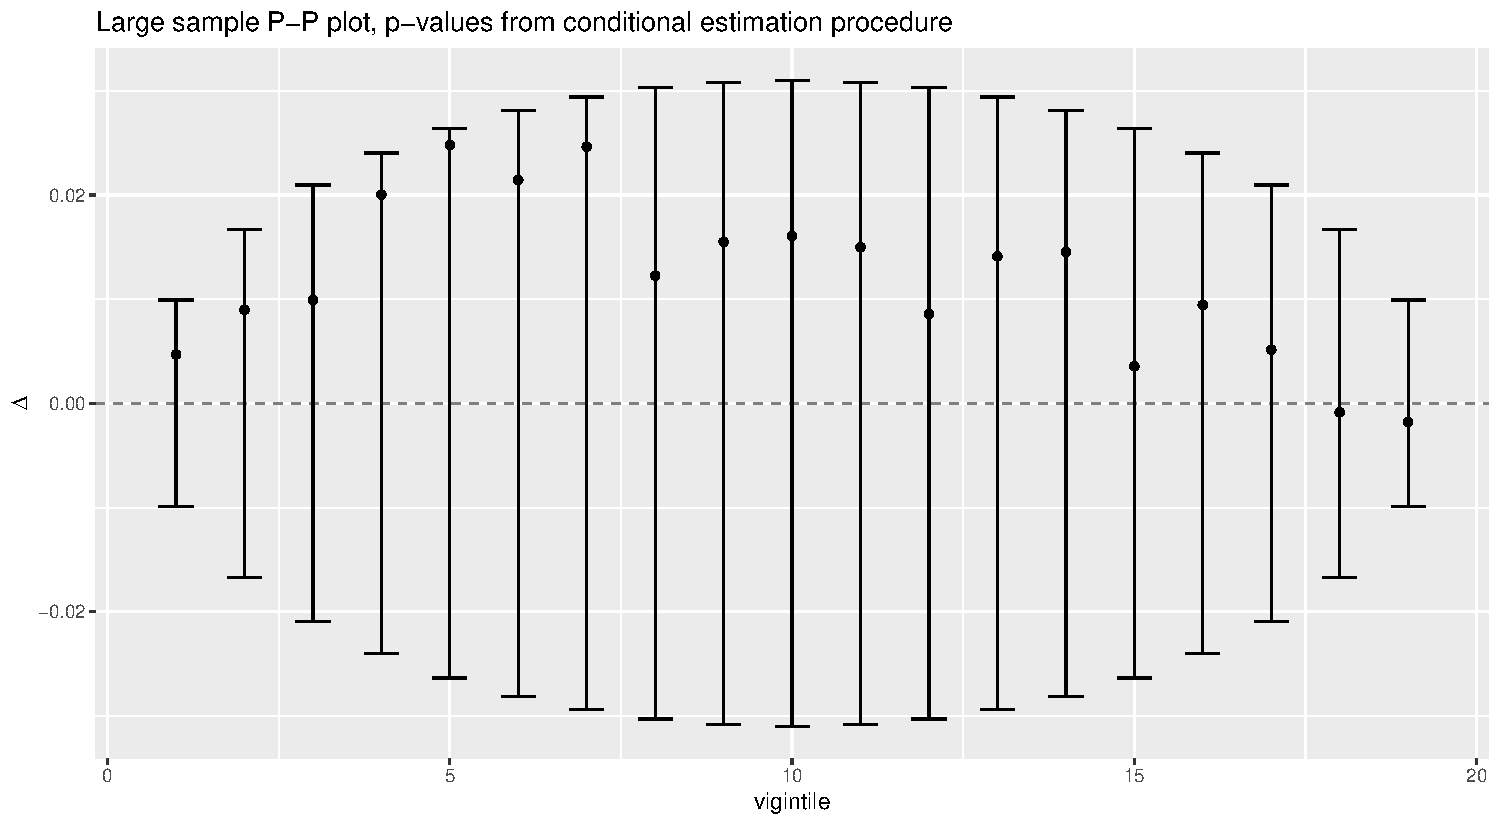
\includegraphics[width=0.975\textwidth]{figure/maxsharpe_motherload_sims_hidden_plotz-1} \caption[The computed p-values from the conditional estimation procedure over 1e+05 simulations are plotted against a uniform law, visually confirming that the p-values are nearly uniform]{The computed p-values from the conditional estimation procedure over 1e+05 simulations are plotted against a uniform law, visually confirming that the p-values are nearly uniform.  Simulations use the exact \RMAT and \pvsnr to compute the covariance matrix. To reduce plot size, we only plot every 100th point. At this sampling rate, as with no subsampling, the points show no deviation from the $y=x$ line.}\label{fig:motherload_sims_hidden_plotz}
\end{figure}


\end{knitrout}
\begin{knitrout}\small
\definecolor{shadecolor}{rgb}{0.969, 0.969, 0.969}\color{fgcolor}\begin{figure}[h]
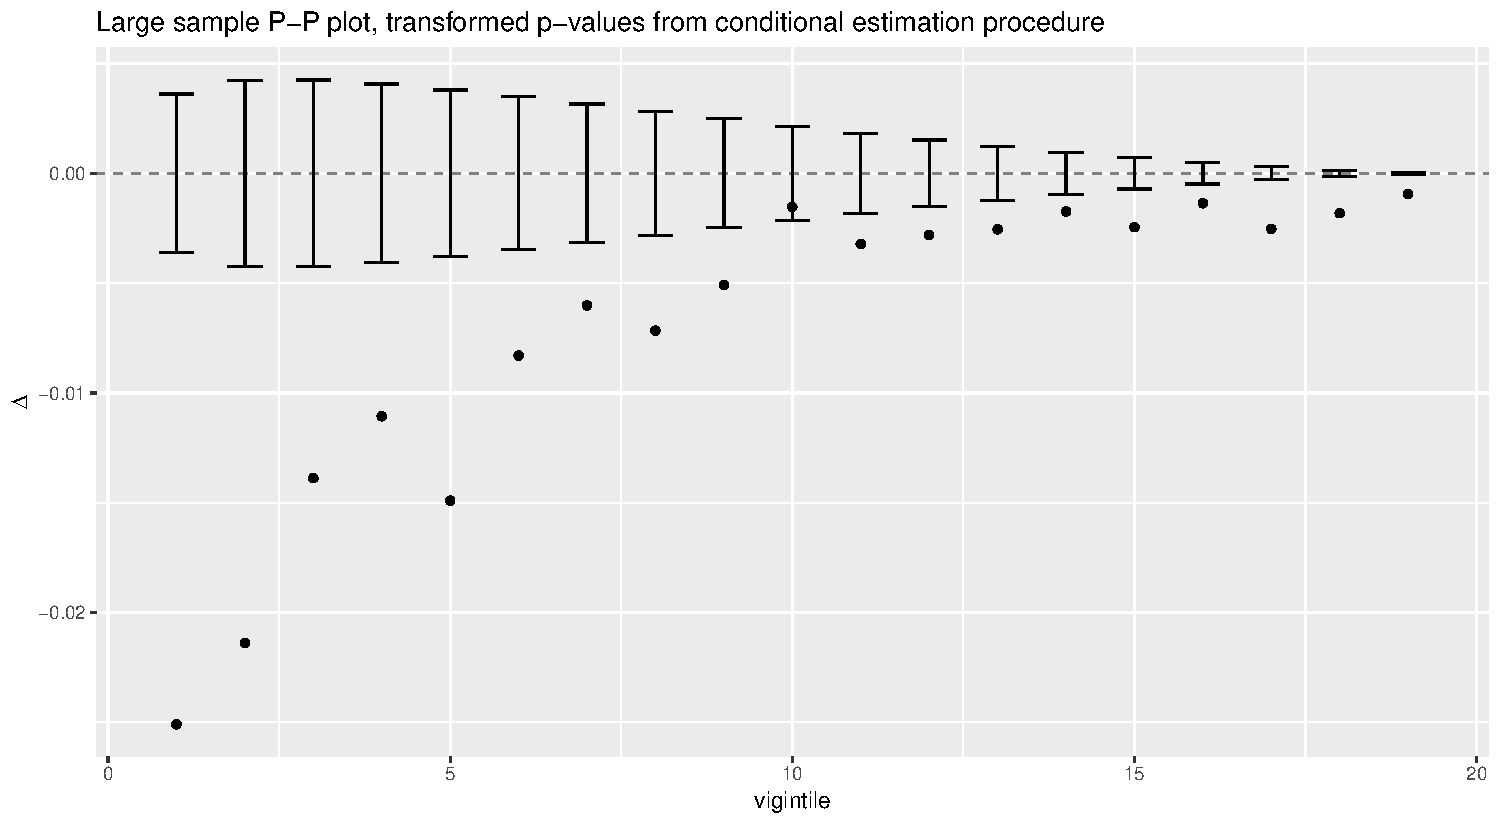
\includegraphics[width=0.975\textwidth]{figure/maxsharpe_motherload_sims_log_plotz-1} \caption{We repeat the P-P plot of \figref{motherload_sims_hidden_plotz}, but in log-log space.  To check uniformity in both tails we compute and plot $p_{*}=2\min\wrapParens{p,1-p}$ versus a uniform distribution.  To reduce plot size, we zoom in on the lower left corner of the P-P plot.}\label{fig:motherload_sims_log_plotz}
\end{figure}


\end{knitrout}
%UNFOLD

\clearpage

\subsubsection{Gaussian returns, feasible estimator}
% causal sims%FOLDUP



While these experiments suggest the normal approximation leads to nearly uniform p-values
under the null, they use the (unknown) population values of \RMAT and \pvsnr to compute
the variance-covariance of \svsr.
So we repeat the experiments, but plug in the usual sample estimate of covariance and the
vector of \txtSRs into \eqnref{apx_srdist_gaussian} to estimate the covariance
matrix of \svsr. 
Other than this change, we repeat the previous experiment, 
performing $\ensuremath{10^{5}}$ simulations, 
setting $\nlatf=100$,
$\RMAT=\makerho{0.7}{0.3}$.
$\ssiz=1260\dayto{}$, \etc
In \figref{causal_sims_log_plotz} we P-P plot the transformed p-value,
$2\min\wrapParens{p,1-p}$ in log-log space.
Again the simulations appear to be uniform.
This is not surprising, because, as noted above, the statistical test
only requires us to estimate the standard error of the \txtSR of the
asset with maximum \txtSR, and so does not greatly rely on the $\nlatf^2$
elements of the estimate of \RMAT.

\begin{knitrout}\small
\definecolor{shadecolor}{rgb}{0.969, 0.969, 0.969}\color{fgcolor}\begin{figure}[h]
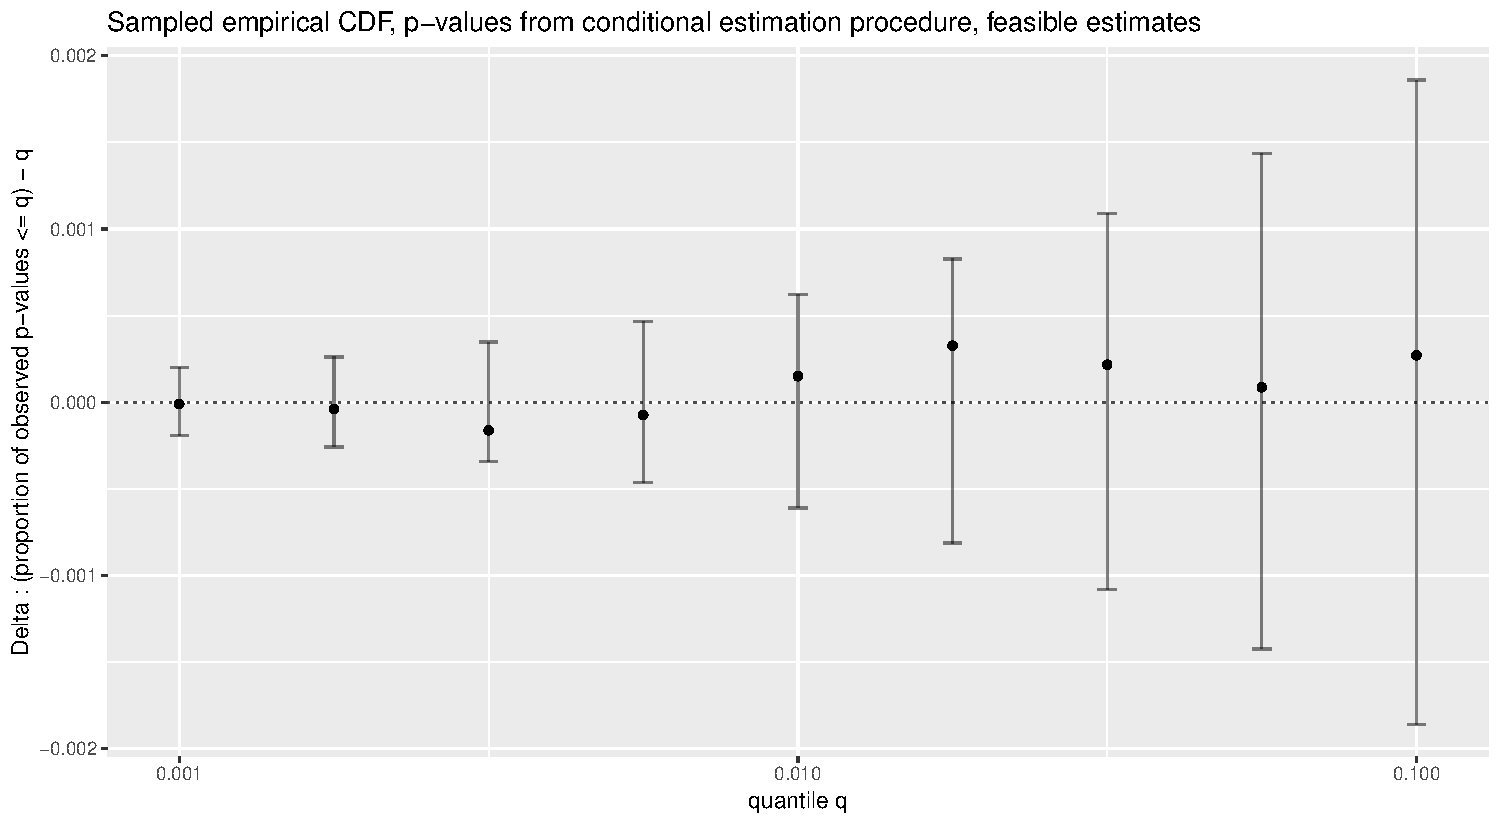
\includegraphics[width=0.975\textwidth]{figure/maxsharpe_causal_sims_log_plotz-1} \caption[P values from the conditional estimation procedure were computed using sample estimates of the covariance matrix, \RMAT, and the vector of \txtSNRs, \pvsnr]{P values from the conditional estimation procedure were computed using sample estimates of the covariance matrix, \RMAT, and the vector of \txtSNRs, \pvsnr. P values $p$ were transformed to $p_{*}=2\min\wrapParens{p,1-p}$, then the $p_{*}$ are P-P plotted against uniformity.  Once again we zoom in on the lower left corner to save plot size.}\label{fig:causal_sims_log_plotz}
\end{figure}


\end{knitrout}
%UNFOLD

\clearpage

\subsubsection{Gaussian returns, feasible estimator, sensitivity}


% many sims with K-S stat?%FOLDUP




This kind of ``proof by eyeball'' is somewhat unsatisfying, and does not scale up to the task
of finding where the approximation is accurate.
To measure the uniformity of our p-values, we generate some via simulations as described above,
then compute the Kolmogorov-Smirnov statistic against a uniform distribution. 
\cite{Marsaglia:Tsang:Wang:2003:JSSOBK:v08i18}
You can think of the K-S statistic as the maximum absolute deviance of a point away
from the $y=x$ line in a P-P plot like 
\figref{motherload_sims_hidden_plotz}.

So we repeat the previous experiments, using a feasible estimator of the covariance matrix of \svsr. 
Again we draw returns from a Gaussian distribution.
We let $\ssiz$ vary from $126$ to $2016$;
we let $\nlatf$ vary from $50$ to $200$;
we let $\rho$ vary from $0$ to $0.8$
where we take 
$\RMAT=\makerho{\rho}{\wrapParens{1-\rho}}$;
we take $\pvsnr$ to be a uniform sequence from $0$ to 
$0.1\dayto{-\halff}$.
For each setting of the parameters in the Cartesian product we perform
$\ensuremath{5\times 10^{4}}$ simulations, computing p values from the feasible estimator.

In \figref{many_sims_plotz} we plot those K-S statistics against $\ssiz$,
with facets for $\rho$ and $\nlatf$. 
All else equal, we expect the approximation to be worse, and thus the K-S statistics
to be higher, for smaller \ssiz and larger \nlatf.
%For the most part this does not seem born out, and there does not seem to be
%a general pattern to the quality of our approximation.
This pattern is somewhat visible in the plots, 
although large $\rho$ seems to reduce the number of `pseudo-assets' in that
relationship.
However, with the given limited evidence,
we cannot claim to have definitively established where our procedure breaks down,
but warn users that the $\nlatf \gg \ssiz$ cases are likely to be problematic
in the sense that nominal type I rates may not be maintained.

\begin{knitrout}\small
\definecolor{shadecolor}{rgb}{0.969, 0.969, 0.969}\color{fgcolor}\begin{figure}[h]
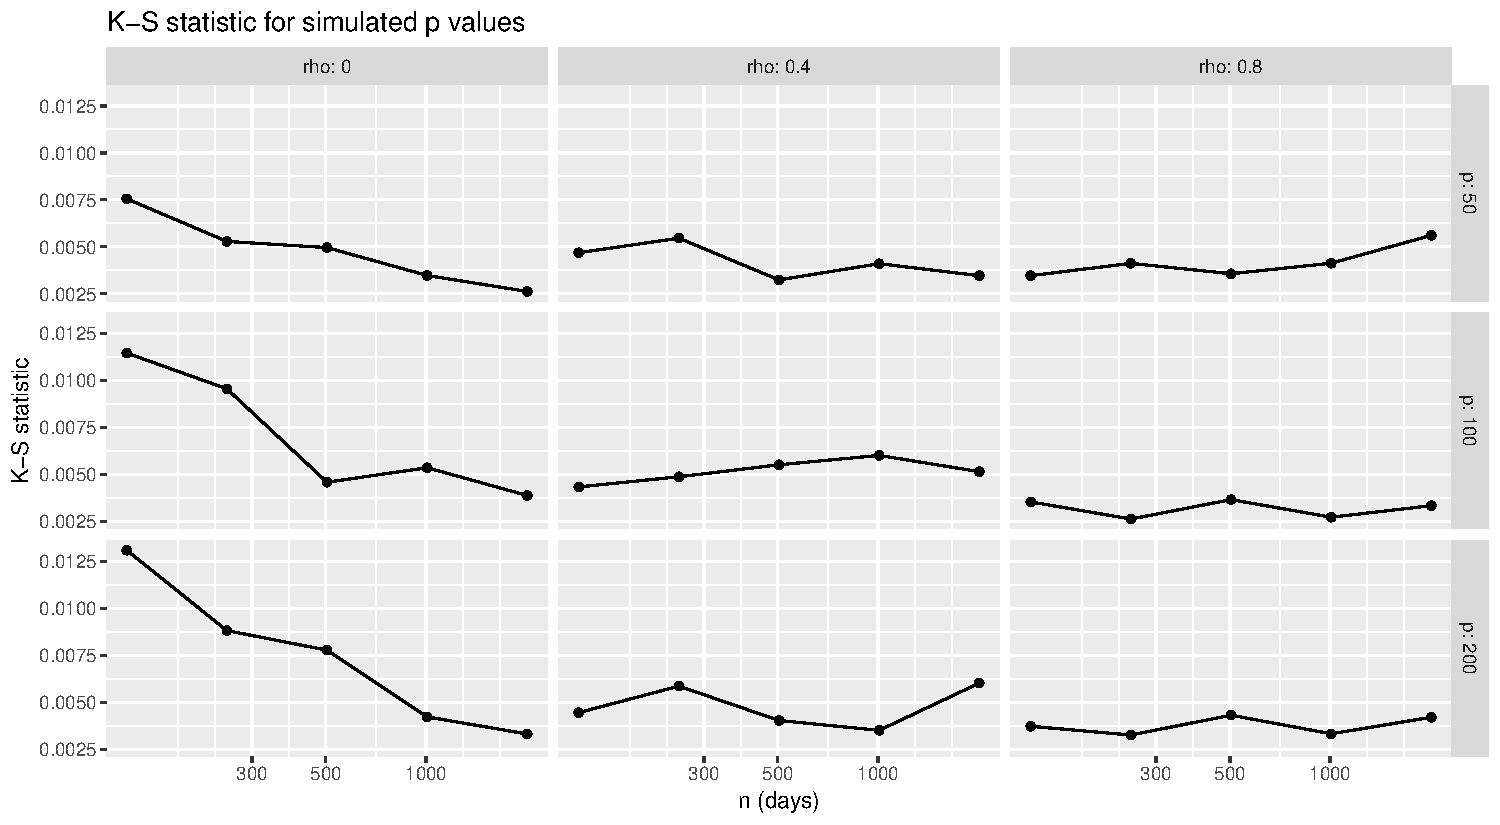
\includegraphics[width=0.975\textwidth]{figure/maxsharpe_many_sims_plotz-1} \caption[Kolmogorov-Smirnov statistics summarizing uniformity of the test statistic $u$ are plotted versus $\ssiz$ with facets for $\nlatf$ and $\rho$]{Kolmogorov-Smirnov statistics summarizing uniformity of the test statistic $u$ are plotted versus $\ssiz$ with facets for $\nlatf$ and $\rho$.  Broadly we see that the test statistic is less uniform in the regime where $\nlatf\gg\ssiz$, but that a large positive $\rho$ perhaps reduces the number of assets in that relationship.}\label{fig:many_sims_plotz}
\end{figure}


\end{knitrout}
%UNFOLD

\subsubsection{$\tstat{}$ returns, feasible estimator}
%FOLDUP


The simulations above were carried out assuming Gaussian returns, and using
\eqnref{apx_srdist_gaussian} to compute the covariance matrix of \svsr.
Gaussian returns are not a good model for real asset returns,
so we repeat those simulations with returns drawn from a multivariate $\tstat{}$-distribution
with $5$ degrees of freedom.  \cite{Lin1972339,kotz2004multivariate}
Again we perform $\ensuremath{10^{4}}$ simulations with
$\nlatf=100$,
$\RMAT=\makerho{0.7}{0.3}$,
$\ssiz=1260\dayto{}$, \etc
We perform inference twice, once using 
\eqnref{apx_srdist_gaussian},
and once using \eqnref{apx_srdist_elliptical} where we have estimated
the kurtosis factor, \kurty, by taking the median of the sample marginal 
kurtosises of the assets. 
In \figref{causal_tfive_sims_plotz} we present the log-space P-P plots
on the transformed p-values under the two methods of estimating
the covariance of \svsr.
There is little difference in the performance of the two sets of simulations. 
We remain cautiously optimistic that for large \ssiz, one need correct
\eqnref{apx_srdist_gaussian} to account for non-normal returns.


\begin{knitrout}\small
\definecolor{shadecolor}{rgb}{0.969, 0.969, 0.969}\color{fgcolor}\begin{figure}[h]
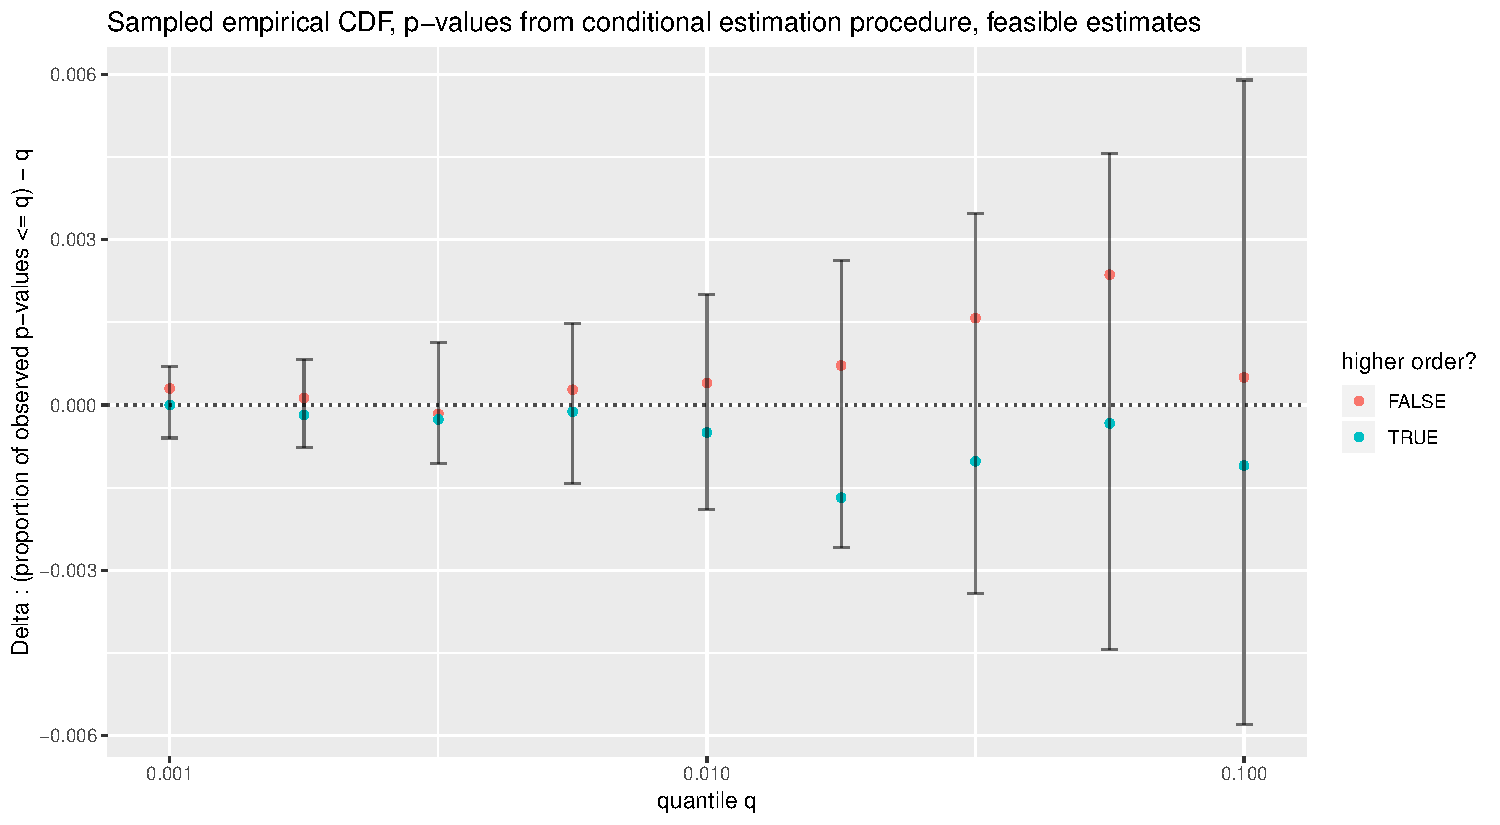
\includegraphics[width=0.975\textwidth]{figure/maxsharpe_causal_tfive_sims_plotz-1} \caption[The computed p-values from the conditional estimation procedure over 10000 simulations are plotted against a uniform law]{The computed p-values from the conditional estimation procedure over 10000 simulations are plotted against a uniform law.  Returns are drawn from a $\tstat{}\wrapParens{5}$ distribution.  Sample estimates are used to construct the variance-covariance matrix of \svsr.  The experiments are performed twice: first assuming that returns are Gaussian; then assuming returns are elliptical with unknown kurtosis factor that we estimate from the sample.  Both procedures give near-uniform p values. Once again we focus on the lower left corner of the plots to trim the plot size.}\label{fig:causal_tfive_sims_plotz}
\end{figure}


\end{knitrout}
%UNFOLD

\clearpage

\subsection{Simulations under the alternative}

We wish to test the power of the method under the alternative hypothesis.
However, it is hard to state exactly what constitutes the alternative.
One interpretation is that we condition on $\psnr[1] > 0$, where again
the indexing is such that $\ssr[1]$ was the maximum over $\nlatf$ assets;
then we estimate the probability of (correctly) rejecting $\psnr[1] = 0$
versus $\psnr[1]$. However, we suspect that the power, as described in 
this way, would depend on the distribution of
values of \pvsnr.

We will consider two extremes: one where all \nlatf elements of \psnr are
equal (``all equal''), and one where $m$ of \nlatf elements of \psnr
are equal to some positive value, and the remaining $\nlatf - m$ are negative
that value (``m-good''), mostly for the case where $m=1$ or $\nlatf = 2m$, which
we call ``half-good''.

% power vs the MHT?




We compare the power of the conditional estimation procedure to that of a
simple MHT correction:
In our experiments, we 
draw returns from a Gaussian distribution with diagonal covariance.
Under this assumption, one can use the distribution of the \tstat{} statistic
to perform inference on the \txtSNR. \cite{pav_ssc}
We then use a simple Bonferroni correction to account for the multiple tests
performed.

Note that in the all equal case, since every asset has the same \txtSNR,
whichever we select will have the same \txtSNR, and the test should have the
same power as the \tstat{}-test for a single asset. 
The conditional estimation procedure, however, may suffer in this case as
we may condition on a \ssr[1] that is very close to being non-optimal,
resulting in a small test statistic for which we do not reject.
On the other hand, for the one-good case, as the $\nlatf - 1$ assets 
may have considerably negative \txtSNR, they are unlikely to exhibit the
largest \txtSR, and so the MHT is merely testing a single asset, but
at the $\typeI / \nlatf$ level instead of the $\typeI$ level, resulting
in lower power. The conditional estimation procedure, however, should
not suffer in this test.

In fact, this is what we see. We perform simulations under all equal, one-good,
and half-good configurations, letting the `good' \txtSNR vary from 
$0$ to $0.15\dayto{-\halff}$, which corresponds
to an `annualized' \txtSNR of around
$2.4\yrto{-\halff}$.
We draw Gaussian returns with diagonal covariance for
$100$ assets, with $\ssiz=1008$.
For each setting we perform $\ensuremath{10^{4}}$ simulations then 
compute the empirical rejection rate of the test at the $0.05$ level,
conditional on the \txtSNR of the \emph{selected} asset, which is
to say the one with the largest \txtSR. Note that in some simulations
the largest \txtSR is observed in an asset with a negative \txtSNR.
We hope our tests to have lower power when this occurs.

In \figref{power_plotz_one}, we plot the power of the MHT Bonferroni
test and the conditional estimation procedure versus the \txtSNR
of the selected asset. 
We present facet columns for the three configurations, 
\viz all equal, one-good, half-good.
A horizontal line at $0.05$ gives the nominal rate under the null,
which occurs as $x=0$ in these plots.
As expected from the above explanation, MHT has higher
power for all equal, while conditional estimation is superior for
one-good.  
For this case we see little difference in performance for 
half-good and all equal.

\begin{knitrout}\small
\definecolor{shadecolor}{rgb}{0.969, 0.969, 0.969}\color{fgcolor}\begin{figure}[h]
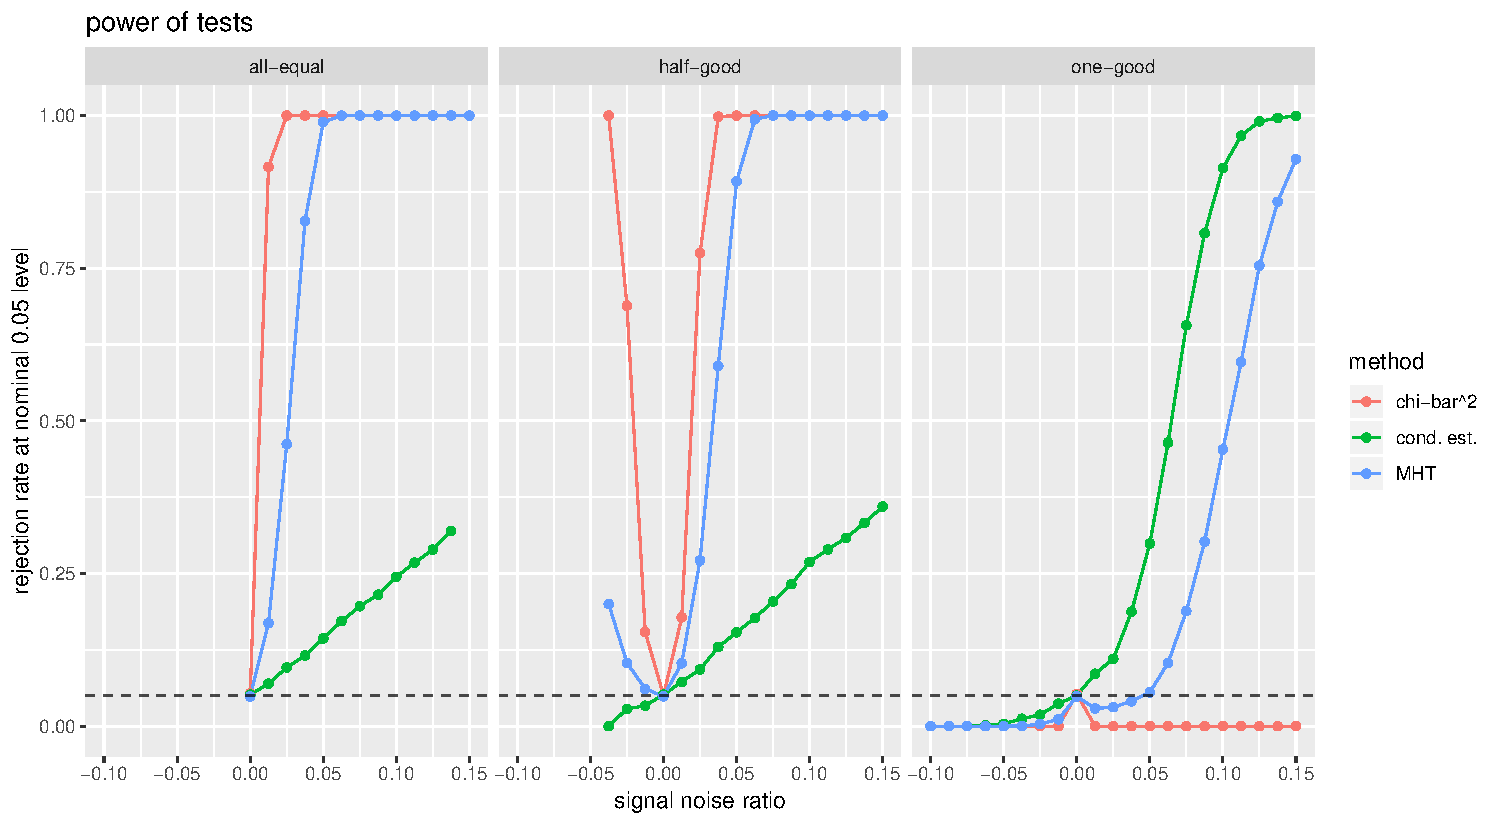
\includegraphics[width=0.975\textwidth]{figure/maxsharpe_power_plotz_one-1} \caption[The empirical power of the conditional estimation and MHT corrected tests are shown versus the \txtSNR of the asset with maximum \txtSR under different arrangements of the vector \pvsnr]{The empirical power of the conditional estimation and MHT corrected tests are shown versus the \txtSNR of the asset with maximum \txtSR under different arrangements of the vector \pvsnr.}\label{fig:power_plotz_one}
\end{figure}


\end{knitrout}


The power of the conditional estimation procedure for the all equal
case is rather disappointing. 
For the case where all assets have a \txtSNR of
$2.4\yrto{-\halff}$,
the test has a power of only around a half.
The test suffers from low power because we are conditioning on
``\ssr[1] is the largest \txtSR'', where we should actually
be conditioning on ``the asset with the largest \txtSR.''

Note the odd plot in the half good facet: the MHT has greater
than $0.05$ rejection rate for \emph{negative} \txtSNR. 
The plot is somewhat misleading in this case, however.
We have performed
$\ensuremath{10^{4}}$ simulations for each setting of the `good'
\txtSNR; in some very small number of them for the half good
case, an asset with negative \txtSNR exhibits the maximum
\txtSR. 
We are plotting the rejection rate for MHT in this case.
But note that the null hypothesis that MHT is testing
\emph{is} violated in this case, because half the assets
have positive \txtSNR, and the MHT tests the null that all
assets have zero or lower \txtSNR.
We have not shown the probability that a `bad' asset has the
highest \txtSR, but note that when the `good' \txtSNR
is greater than $0.05\dayto{-\halff}$ we do not observe this
occuring even once over the $\ensuremath{10^{4}}$ simulations performed
for each setting. 
This does indicate, however, that the simple settings of the 
spread of \pvsnr we tested here are unlikely to have revealed 
all the relevant differences between the two tests or their
deficiencies in certain situations.


\subsubsection{Simulations under the null versus with correlated returns}



On the other hand, the MHT test cannot maintain the nominal type I rate in the face of correlated assets.
To demonstrate this, we repeat the experiments above, but setting 
$\RMAT=\makerho{\rho}{\wrapParens{1-\rho}}$
and $\psnr=\vzero$.
Again we consider $\nlatf=100$, 
$\ssiz=1008$, and perform $5000$ simulations to estimate the 
empirical rejection rate.
In \figref{rho_plotz_one}, we plot the empirical rejection rate versus $\rho$ at the nominal
$0.05$ type I level. 
While the conditional estimation procedure appears to maintain the nominal rejection
rate, even though \RMAT is being estimated from the sample,
the MHT test is conservative, with near zero rejection rates for large $\rho$.
The fix for common correlation described in \subsecref{fix_bonferroni} is also tested,
yielding nominal rejection rates.
%If \svsr were normally distributed, which is a fair approximation, this would be guaranteed
%by Slepian's Lemma, which tells us that for a normally distributed Gaussian vector
%with fixed mean and variance, the maximum element is `stochastically decreasing' in the correlation.  \cite{slepian1962one}
%Intuitively, the number of `pseudo assets' is reduced when returns have higher correlation, and
%the Bonferroni correction is too conservative.

\begin{knitrout}\small
\definecolor{shadecolor}{rgb}{0.969, 0.969, 0.969}\color{fgcolor}\begin{figure}[h]
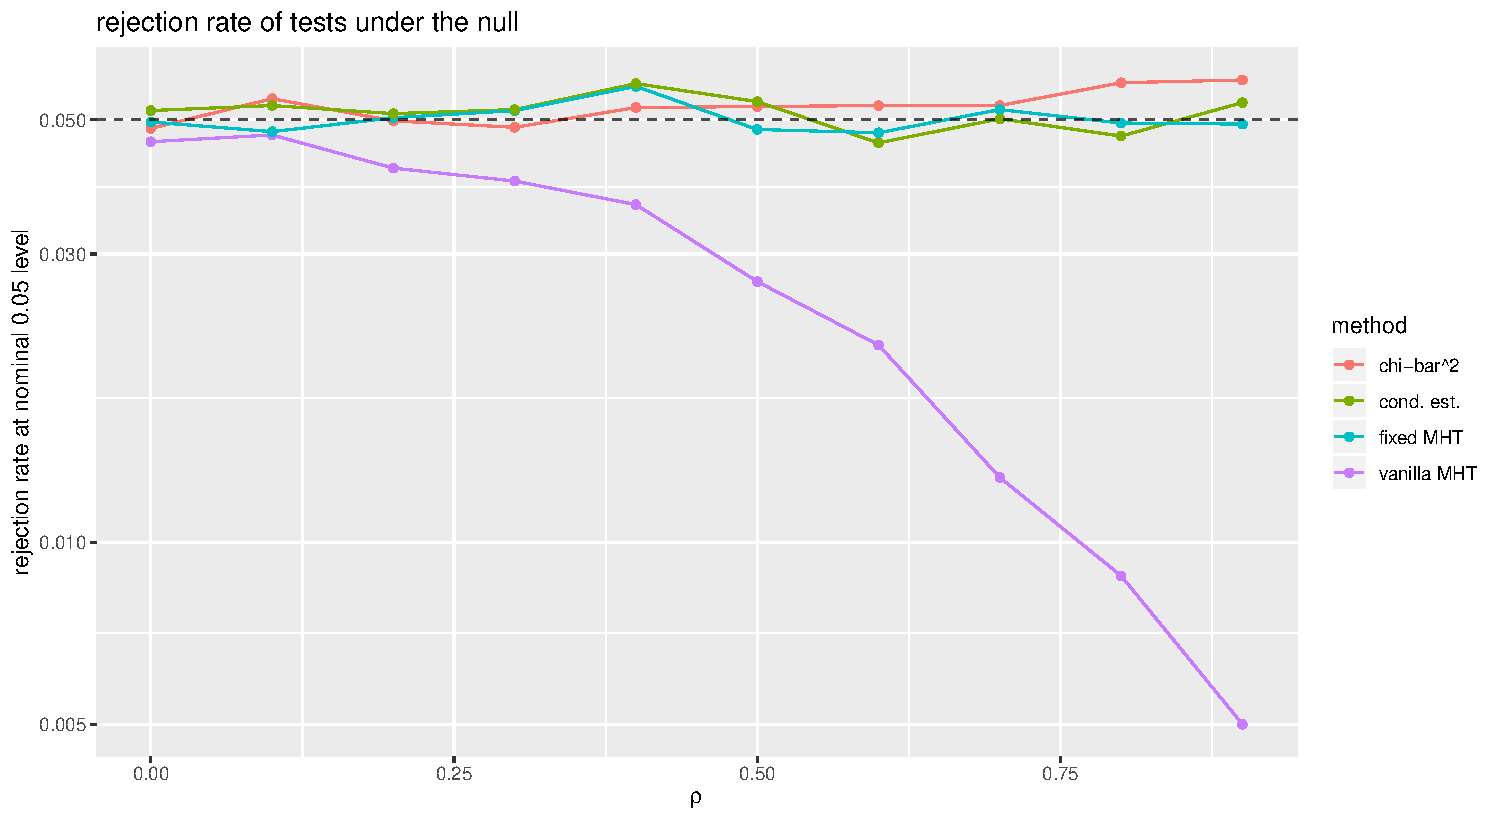
\includegraphics[width=0.975\textwidth]{figure/maxsharpe_rho_plotz_one-1} \caption[The empirical type I rate under the null hypothesis is plotted versus $\rho$ for the case where $\RMAT=\makerho{\rho}{\wrapParens{1-\rho}}$, for three testing procedures]{The empirical type I rate under the null hypothesis is plotted versus $\rho$ for the case where $\RMAT=\makerho{\rho}{\wrapParens{1-\rho}}$, for three testing procedures: the conditional estimation, vanilla Bonferroni correction, and Bonferroni correction with fix for common correlation.  Tests are performed with Gaussian returns, for 100 assets over 1008 days. Tests were performed at the $0.05$ level, which appears to be maintained by the conditional estimation and fixed Bonferroni procedures but not by the regular Bonferroni procedure.  Empirical rates are over 5000 simulations. The $y$ axis is in log scale.}\label{fig:rho_plotz_one}
\end{figure}


\end{knitrout}

%UNFOLD

\clearpage

\subsection{Five Industry Portfolios}

% 2FIX: start from here ... 


We download the monthly returns of five industry portfolios
from Ken French's data library. \cite{ind_5_def}
%These consist of 
We consider the 1104 months of data on five industries
from Jan 1927 to Dec 2018.
We compute the \txtSR of the returns of each, and present them
in \tabref{mind_sr}. 
We have reordered the industries in decreasing \txtSR.
The industry portfolio with the highest \txtSR was
Healthcare with a \txtSR of 
around $0.193\,\moto{-\halff}$ which is approximately
$0.667\,\yrto{-\halff}$.

% latex table generated in R 3.3.2 by xtable 1.8-2 package
% Sat Jun  8 21:42:47 2019
\begin{table}[ht]
\centering
\begin{tabular}{r|c}
  \hline
industry & Sharpe Ratio \\ 
  \hline
Healthcare & $ 0.193\,\moto{-\halff} $ \\ 
  Consumer & $ 0.187\,\moto{-\halff} $ \\ 
  Manufacturing & $ 0.172\,\moto{-\halff} $ \\ 
  Technology & $ 0.170\,\moto{-\halff} $ \\ 
  Other & $ 0.140\,\moto{-\halff} $ \\ 
   \hline
\end{tabular}
\caption{The \txtSRs of the five industry portfolios are shown.} 
\label{tab:mind_sr}
\end{table}




We are interested in computing $95\%$ upper confidence
intervals on the \txtSNR of the Healthcare portfolio. 
We are only considering this portfolio as it is the one with maximum \txtSR
in our sample.
If we had been interested in testing
Healthcare 
without our conditional selection, we would compute the confidence interval
$\left[0.143\,\moto{-\halff}, \infty\right)$ based on inverting the non-central
\tstat{}-distribution. \cite{pav_ssc,SharpeR-Manual}
If instead we approximate the standard error by plugging in 
$0.193\,\moto{-\halff}$ as the \txtSNR of 
Healthcare 
into \eqnref{apx_srdist_gaussian},
we estimate the standard error of the \txtSR to be
$0.03\,\moto{-\halff}$.
Based on this we can compute the na\"{i}ve confidence interval of
the measured \txtSR plus 
$\qnorm{0.05}=-1.645$ times the standard error.
This also gives the confidence interval
$\left[0.143\,\moto{-\halff}, \infty\right)$.

Using the simple Bonferroni correction, however, since we selected
Healthcare 
only for having the maximum \txtSR, we should compute the 
confidence interval by adding
$\qnorm{0.01}=-2.326$ times the standard error.
This yields the confidence interval
$\left[0.122\,\moto{-\halff}, \infty\right)$.

The correlation of industry returns is high, however.
The pairwise sample correlations range from
0.708 to 
0.891 with a median value of
0.801.
Plugging this value in as $\rho$, 
we find the value $c$ such that the $z_1$ from \eqnref{fix_bonf_z}
is equal to 
$\qnorm{0.01}=-2.326$.
This leads to the confidence interval 
$\left[0.125\,\moto{-\halff}, \infty\right)$.

Finally we use the conditional estimation procedure, inverting
the hypothesis test to find the corresponding population value.
This yields the confidence interval 
$\left[0.073\,\moto{-\halff}, \infty\right)$.


%%%%%%%%%%%%%%%%%%%%%%%%%%%%%%%%%%%%%%%%%%%%%%%%%%%%%%%%%%%%%%%%%%%%%%%%
\section{Conclusions and Future Work}%FOLDUP

The conditional estimation procedure appears to achieve nominal
type I rates under the null, and does not seem unduly harmed by assuming
the vector \svsr is normally distributed. 
Nor does it seem to suffer greatly from using sample estimates
of the correlation matrix, \RMAT, nor from the presence of 
kurtotic returns.
The procedure can be used for other test configurations beyond the
asset with the maximum \txtSR,
and can be used to construct confidence intervals.
However, it appears to have low power when many assets have the
same \txtSNR.

Clearly the low power of the test gives us reason to seek improvements.
Perhaps the conditioning procedure can be adapted to recognize
that the strategist would have been testing another asset if the
\txtSR of the currently selected asset had been lower. 
Perhaps the power of the MHT for the case of equal \txtSNRs can
be somehow ported to the conditional estimation procedure, perhaps
by testing multiple 
assets\footnote{Note that White's Reality Check and Hansen's SPA
appear to avoid this issue by comparing the maximum in-sample 
predictive ability to the \emph{average} predictive ability of
tested models.  \cite{White:2000,Hansen:2005}}.
Finally, the fix for Bonferroni correction under rank-one updated
correlation \RMAT can potentially be generalized to deal
with more realistic correlation matrices.

%Lastly we mention that when asset returns are well approximated
%by a linear combination of $k$ `latent' returns, we can
%view the asset with maximum \txtSR as holding the sample \txtMP
%over the latent returns, then appeal to the theory of the
%statistic of the \txtMP via Hotelling's $T^2$ statistic.  \cite{pav_maxsharpe_two}
%This approach requires further development.
%UNFOLD

%%%%%%%%%%%%%%%%%%%%%%%%%%%%%%%%%%%%%%%%%%%%%%%%%%%%%%%%%%%%%%%%%%%%%%%%
% bibliography%FOLDUP
%\nocite{markowitz1952portfolio,markowitz1999early,markowitz2012foundations}
%\bibliographystyle{jss}
%\bibliographystyle{siam}
%\bibliographystyle{ieeetr}
\bibliographystyle{plainnat}
%\bibliographystyle{acm}
%\bibliography{SharpeR,rauto}
\bibliography{common}
%\bibliography{AsymptoticMarkowitz}
%UNFOLD

%%%%%%%%%%%%%%%%%%%%%%%%%%%%%%%%%%%%%%%%%%%%%%%%%%%%%%%%%%%%%%%%%%%%%%%%
\appendix%FOLDUP

\section{Establishing \eqnref{apx_srdist_elliptical}.}


Let \Mtx{V} be the variance covariance to be computed. Then from
\eqnref{delmethod}, 
\begin{align*}
  \Mtx{V} &= \qoform{\pvvar}{\wrapParens{\dbyd{\pvsnr}{\vcat{\pvmu}{\pvmom[2]}}}},\\
   &= 
   \Mdiag{\frac{1}{\pvsigma^2}}
\onebytwo{\Mdiag{\pvsigma + \pvmu\pvsnr}}{
  {\Mdiag{\frac{- \pvsnr}{2}}}} 
  \pvvar
\twobyone{\Mdiag{\pvsigma + \pvmu\pvsnr}}{
  {\Mdiag{\frac{- \pvsnr}{2}}}} 
   \Mdiag{\frac{1}{\pvsigma^2}}.
\end{align*}

Plugging in \pvvar from \eqnref{elliptical_variances}, we have
\begin{align*}
  \Mtx{V} &= 
   \Mdiag{\frac{1}{\pvsigma^2}}
   \left\{
\Mdiag{\pvsigma + \pvmu\pvsnr}
\pvsig
\Mdiag{\pvsigma + \pvmu\pvsnr}
+ 
\Mdiag{\pvsigma + \pvmu\pvsnr}
2\pvsig\Mdiag{\pvmu}
\Mdiag{\frac{- \pvsnr}{2}}
   \right.\\
   &\phantom{=\Mdiag{\frac{1}{\pvsigma^2}}}\,
   \left.
+\Mdiag{\frac{- \pvsnr}{2}}
2\Mdiag{\pvmu}\pvsig
\Mdiag{\pvsigma + \pvmu\pvsnr}
+
\Mdiag{\frac{- \pvsnr}{2}}
2 \pvsig \hadm \pvsig
\Mdiag{\frac{- \pvsnr}{2}}\right.\\
   &\phantom{=\Mdiag{\frac{1}{\pvsigma^2}}}\,
   \left.
+
\Mdiag{\frac{- \pvsnr}{2}}
	4 \Mdiag{\pvmu}\pvsig\Mdiag{\pvmu}
\Mdiag{\frac{- \pvsnr}{2}}
   \right\}
   \Mdiag{\frac{1}{\pvsigma^2}},\\
  &= 
   \Mdiag{\frac{1}{\pvsigma^2}}
   \left\{
 \Mdiag{\pvsigma}
\pvsig
  \Mdiag{\pvsigma}
-
\Mdiag{\pvmu\pvsnr}
\pvsig
\Mdiag{\pvmu\pvsnr}\right.\\
   &\phantom{=\Mdiag{\frac{1}{\pvsigma^2}}}\,
   \left.
+
\Mdiag{\frac{- \pvsnr}{2}}
2 \pvsig \hadm \pvsig
\Mdiag{\frac{- \pvsnr}{2}}\right.\\
   &\phantom{=\Mdiag{\frac{1}{\pvsigma^2}}}\,
   \left.
+
\Mdiag{\pvmu\pvsnr}
\pvsig
\Mdiag{\pvmu\pvsnr}
   \right\}
   \Mdiag{\frac{1}{\pvsigma^2}},\\
&=
   \Mdiag{\frac{1}{\pvsigma^2}}
   \wrapBraces{
 \Mdiag{\pvsigma}
\pvsig
  \Mdiag{\pvsigma}
  + \half
\Mdiag{\pvsnr}
\pvsig \hadm \pvsig
\Mdiag{\pvsnr}}
   \Mdiag{\frac{1}{\pvsigma^2}},\\
&=
\RMAT 
+ \half
\Mdiag{\pvsnr}
   \Mdiag{\frac{1}{\pvsigma^2}}
\pvsig \hadm \pvsig
   \Mdiag{\frac{1}{\pvsigma^2}}
\Mdiag{\pvsnr},\\
&=
\RMAT 
+ \half
\Mdiag{\pvsnr}
\RMAT \hadm \RMAT
   \Mdiag{\frac{1}{\pvsigma^2}}.
\end{align*}
%UNFOLD

Proving \eqnref{apx_srdist_elliptical} is similar, and is left as an exercise for the reader.

\end{document}
%for vim modeline: (do not edit)
% vim:fdm=marker:fmr=FOLDUP,UNFOLD:cms=%%s:syn=tex:ft=tex:et:nu:tw=151:cole=0:fo=croql
